\documentclass[11pt,a4paper]{article}
\usepackage[utf8]{inputenc}
\usepackage[T1]{fontenc}
\usepackage[margin=2.5cm]{geometry}
\usepackage{parskip}
\usepackage{setspace}
\usepackage{graphicx}
\usepackage{booktabs}
\usepackage{hyperref}
\usepackage{xcolor}
\usepackage{enumitem}
\usepackage{listings}

% ---------------- Listings (Python) ----------------
\lstdefinestyle{pythonstyle}{
    language=Python,
    basicstyle=\ttfamily\small,
    showstringspaces=false,
    breaklines=true,
    keywordstyle=\color{blue!70!black},
    stringstyle=\color{teal!60!black},
    commentstyle=\color{gray!70},
    frame=single,
    numbers=left,
    numberstyle=\tiny\color{gray},
    stepnumber=1,
    numbersep=8pt,
    columns=fullflexible
}
\lstset{style=pythonstyle}

\title{\textbf{Laporan Praktikum Mandiri 3: Implementasi Multiple Linear Regression pada Dataset Bike Sharing}}
\author{Rafa Al Razzak \\ NIM: 0110224155 \\ \texttt{0110224155@student.nurulfikri.ac.id}}

\begin{document}
\maketitle
\onehalfspacing

\begin{abstract}
Dokumen ini menyajikan implementasi algoritma Multiple Linear Regression untuk prediksi jumlah penyewaan sepeda menggunakan dataset Bike Sharing dari Kaggle.
Analisis meliputi preprocessing data, analisis korelasi, seleksi fitur, pembagian dataset, pelatihan model, dan evaluasi performa.
Dataset memiliki variabel dependen \texttt{cnt} (total penyewaan sepeda) dan 11 variabel independen yang dipilih berdasarkan korelasi dan relevansi bisnis.
Model yang dihasilkan mencapai akurasi 82.77\% dengan R² Score 0.8277, menunjukkan kemampuan prediksi yang baik untuk aplikasi praktis.
\end{abstract}

\vspace{-1mm}

\section{Pendahuluan}
Multiple Linear Regression adalah algoritma supervised learning yang digunakan untuk memprediksi nilai kontinu berdasarkan multiple variabel independen.
Dataset Bike Sharing dari Kaggle digunakan untuk memprediksi jumlah penyewaan sepeda berdasarkan faktor cuaca, musim, dan temporal.
Implementasi menggunakan library scikit-learn dengan evaluasi menggunakan metrik MSE, RMSE, MAE, dan R² Score.

\section{Memuat Dataset}
Memuat dataset bike sharing yang berisi informasi penyewaan sepeda harian dari tahun 2011--2012.
\begin{lstlisting}[language=Python]
import pandas as pd

df = pd.read_csv("../DATA/day.csv")
df.head()
\end{lstlisting}

\begin{figure}[h]
    \centering
    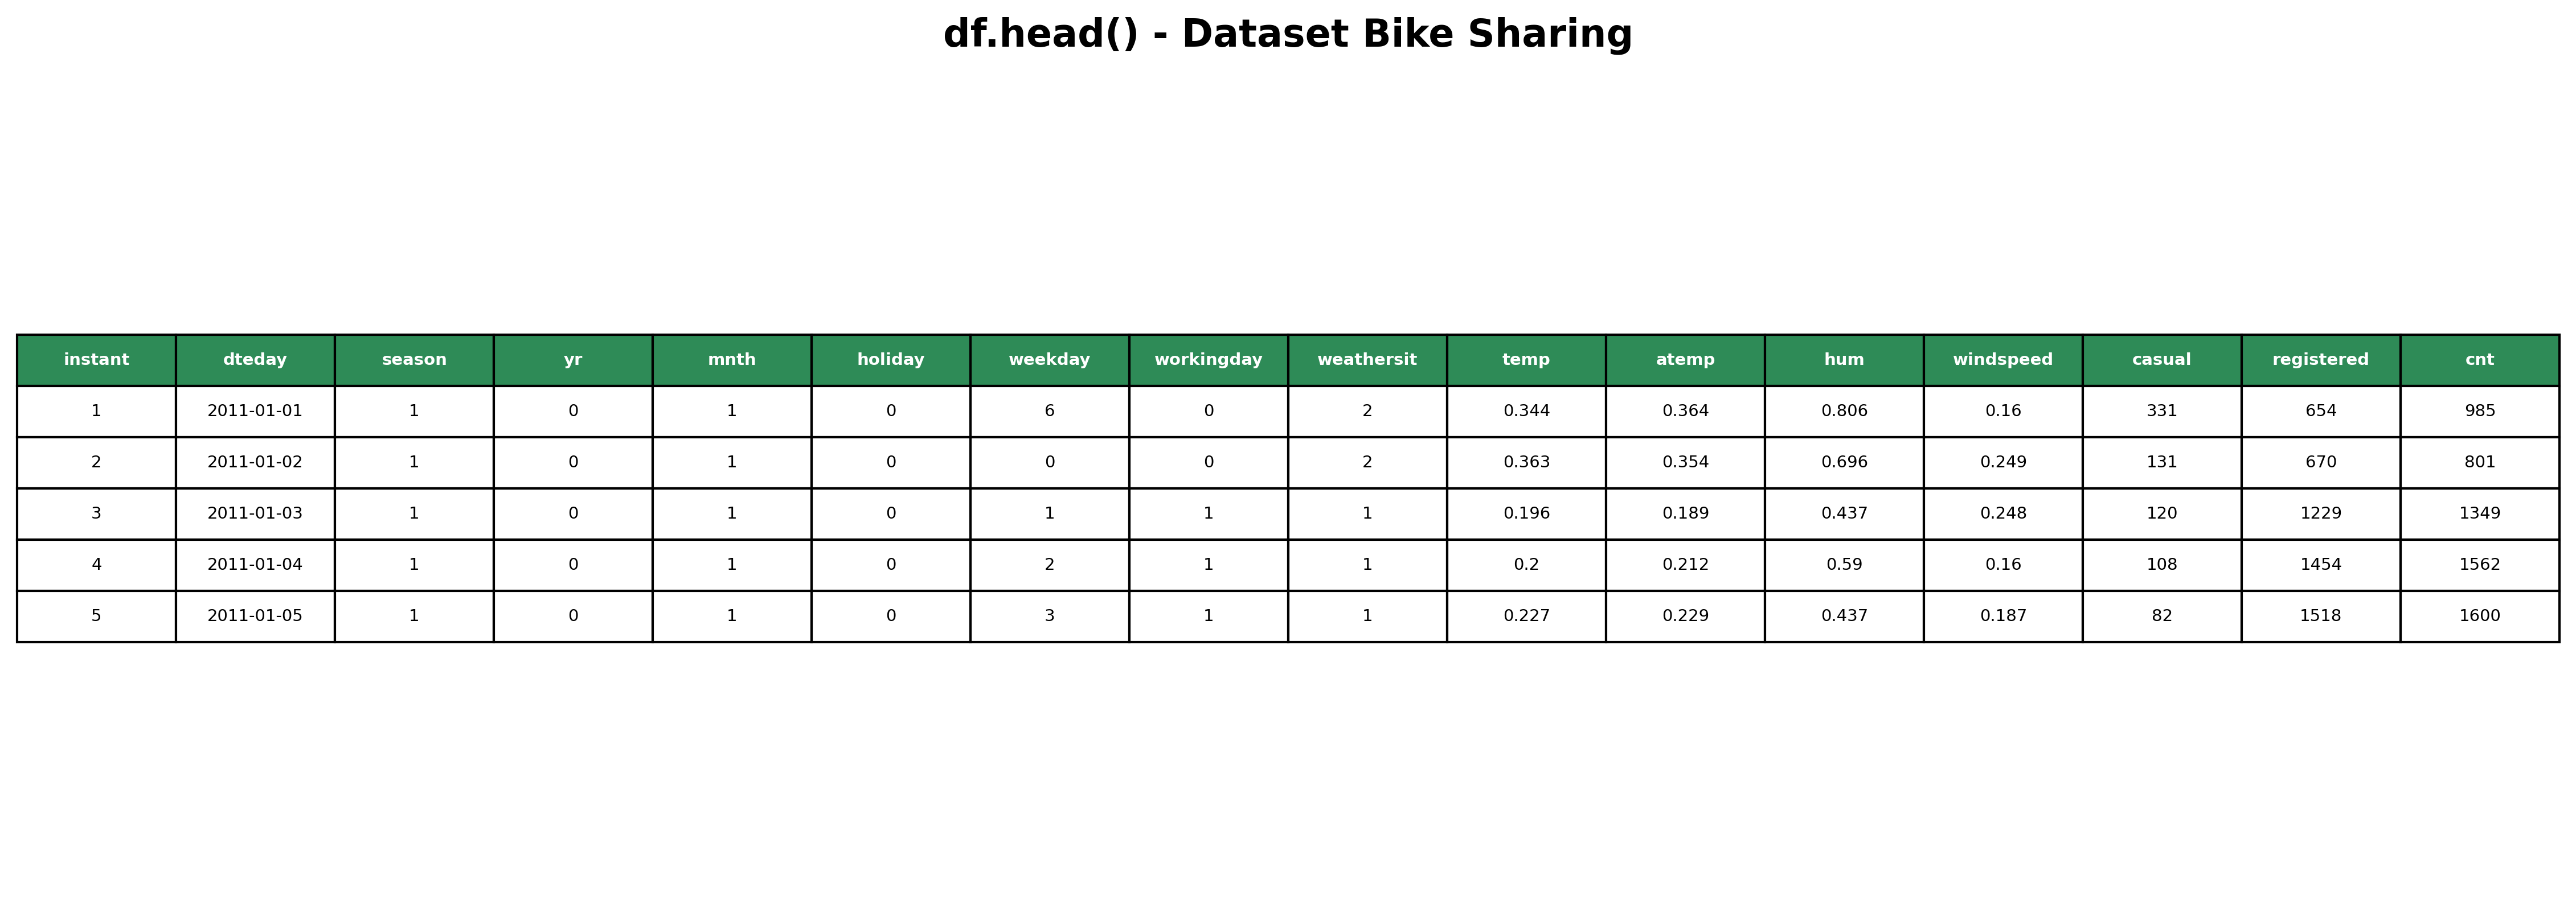
\includegraphics[width=0.8\textwidth]{./OUTPUT/step1_dataset_head.png}
    \caption{Dataset Bike Sharing - Menampilkan 5 Baris Pertama}
    \label{fig:dataset_head}
\end{figure}

\noindent\textbf{Ringkasan Dataset.}
Berisi 731 baris dan 16 kolom dengan data harian 2011--2012. Kolom target adalah \texttt{cnt} (total penyewaan sepeda per hari).

\section{Preprocessing Data}
Melakukan preprocessing dengan menghapus kolom \texttt{instant} dan memformat kolom \texttt{dteday} menjadi \textit{datetime}.
\begin{lstlisting}[language=Python]
# Preprocessing Data
df_processed = (
    df
    .drop(columns=["instant"])
    .assign(
        dteday=lambda x: pd.to_datetime(x["dteday"])
    )
).copy()

print("Info Dataset:")
print(df_processed.info())
print("\nDeskripsi Statistik:")
print(df_processed.describe())
\end{lstlisting}

\begin{figure}[h]
    \centering
    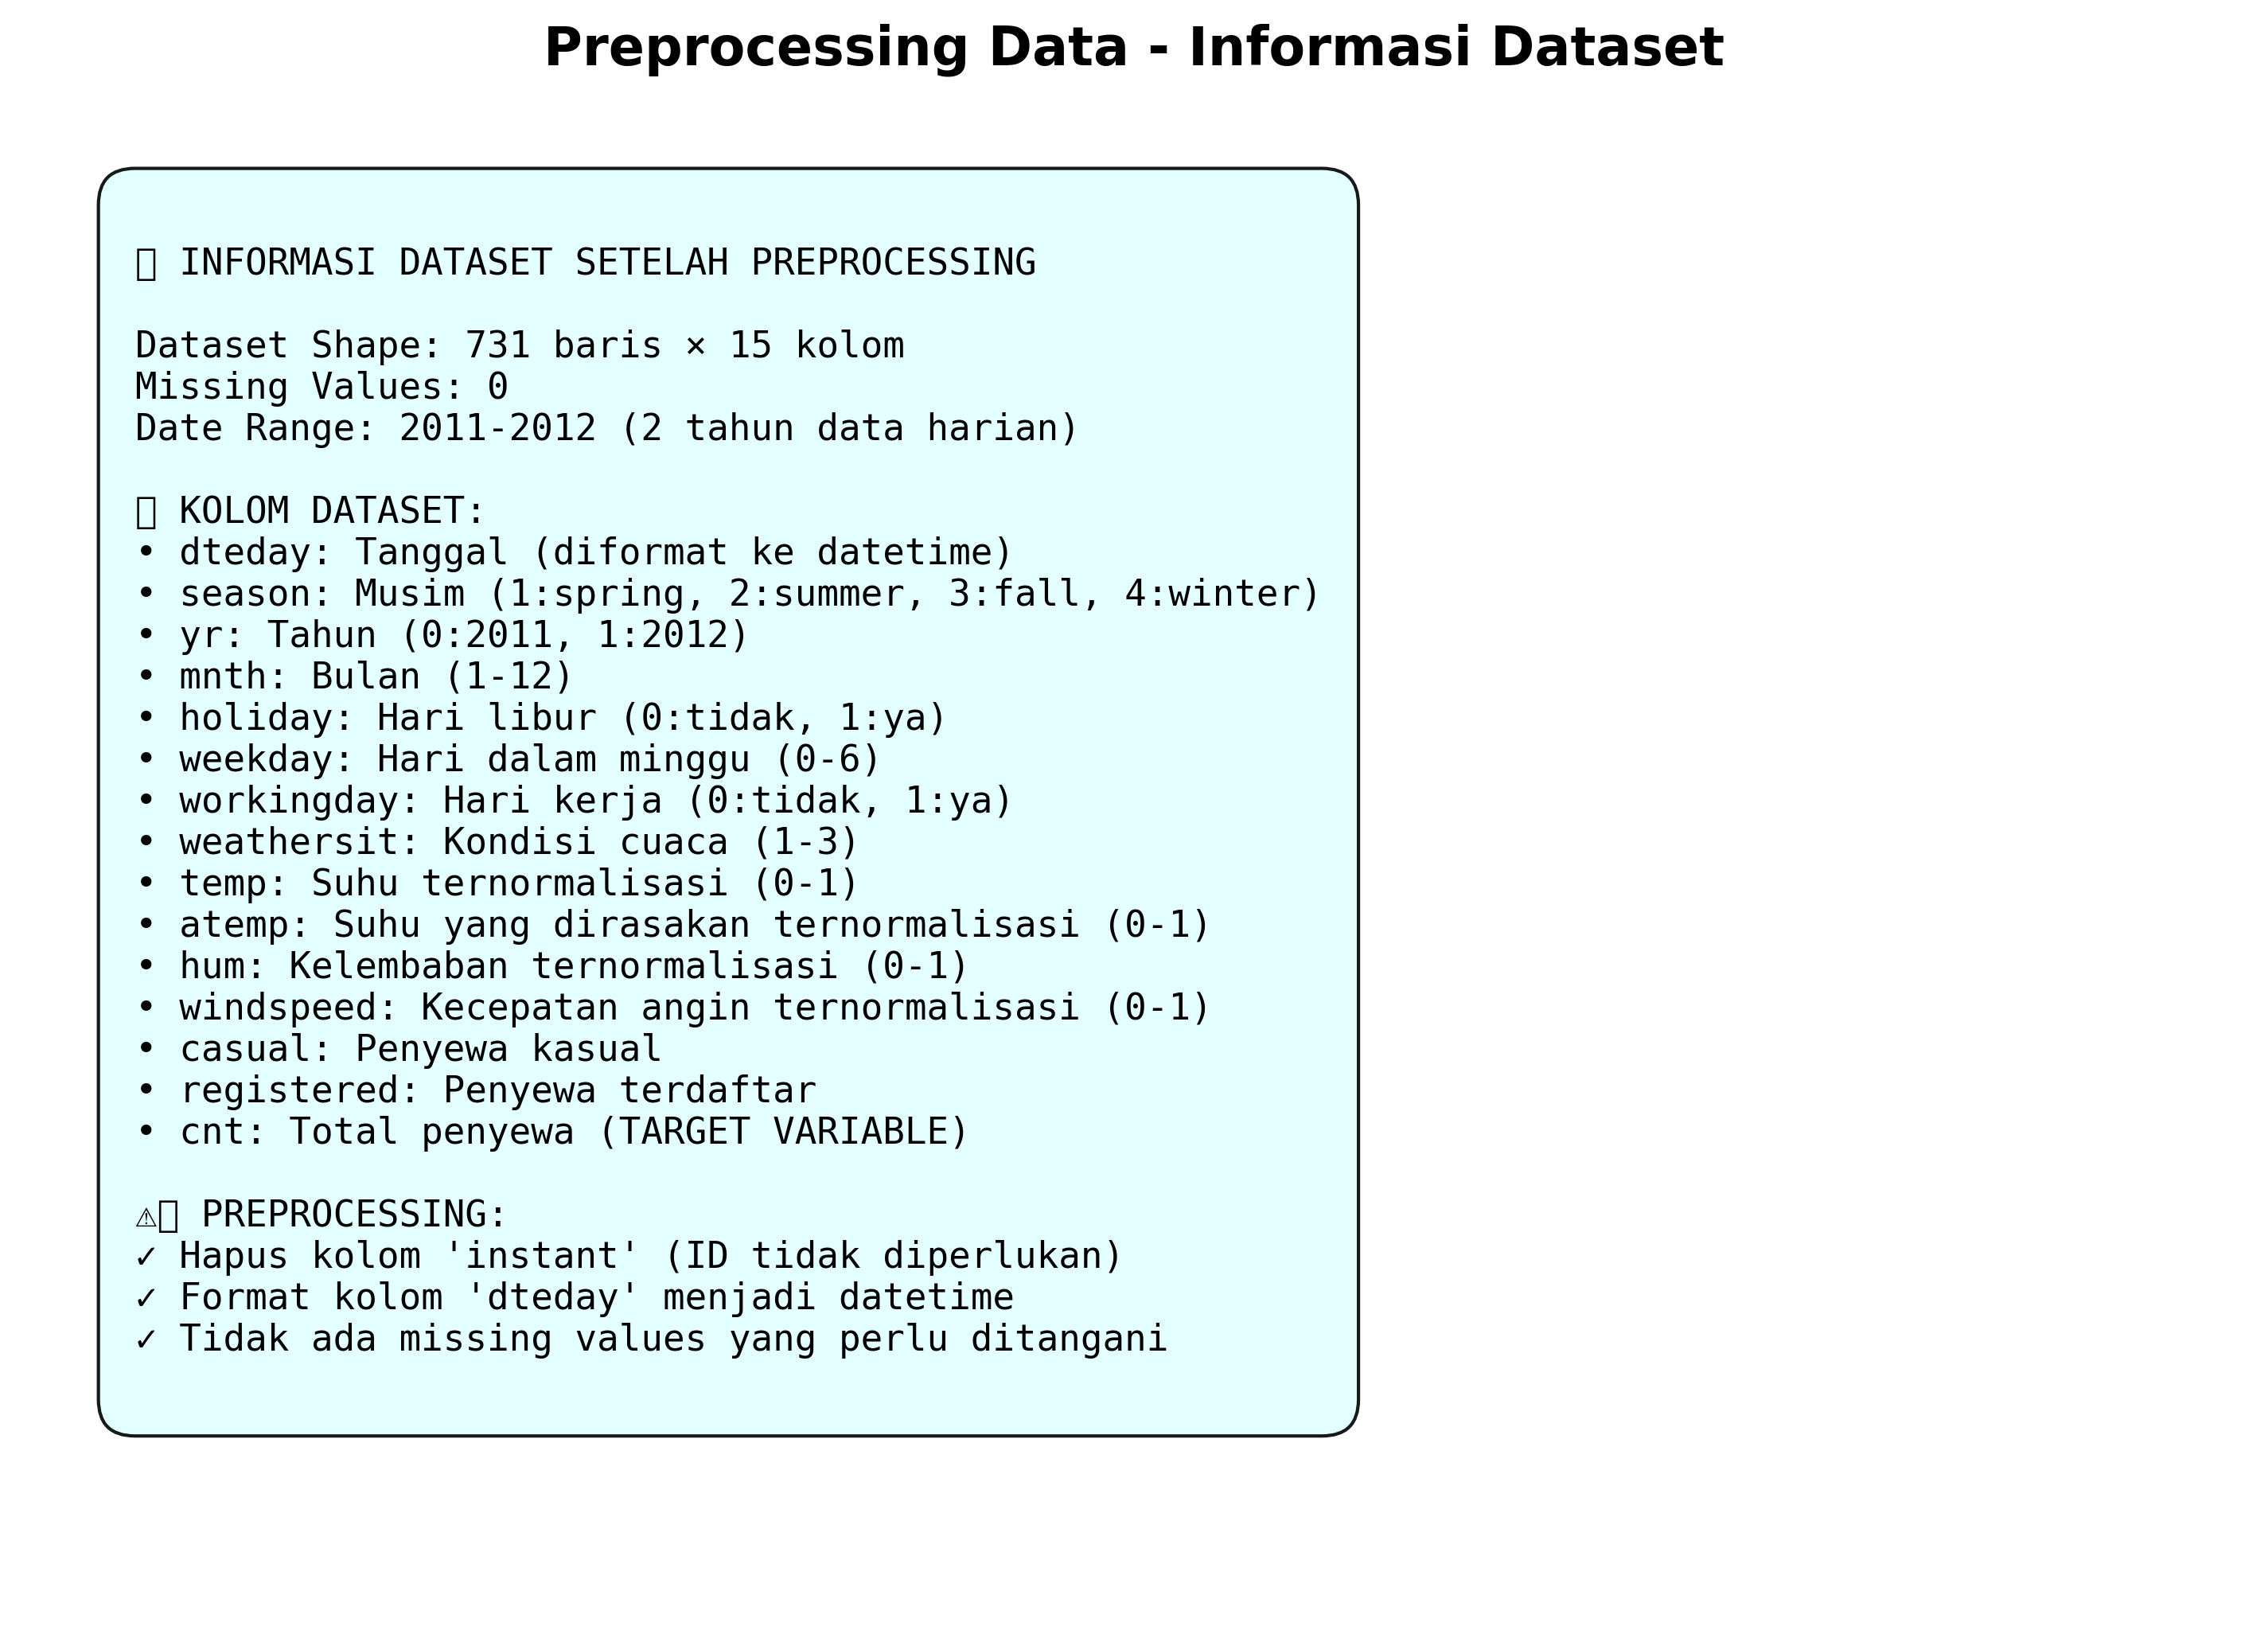
\includegraphics[width=0.85\textwidth]{./OUTPUT/step2_preprocessing_info.png}
    \caption{Informasi Dataset Setelah Preprocessing}
    \label{fig:preprocessing_info}
\end{figure}

\noindent\textbf{Catatan Preprocessing.}
Kolom \texttt{instant} (ID) dihapus; \texttt{dteday} diformat ke \textit{datetime}. Tidak ada \textit{missing values}; tersisa 15 kolom.

\section{Analisis Korelasi}
Menghitung matriks korelasi dan menampilkan 5 baris pertama.
\begin{lstlisting}[language=Python]
# Analisis Korelasi
import matplotlib.pyplot as plt
import seaborn as sns

corr_matrix = df_processed.corr()
corr_matrix.head()
\end{lstlisting}

\begin{figure}[h]
    \centering
    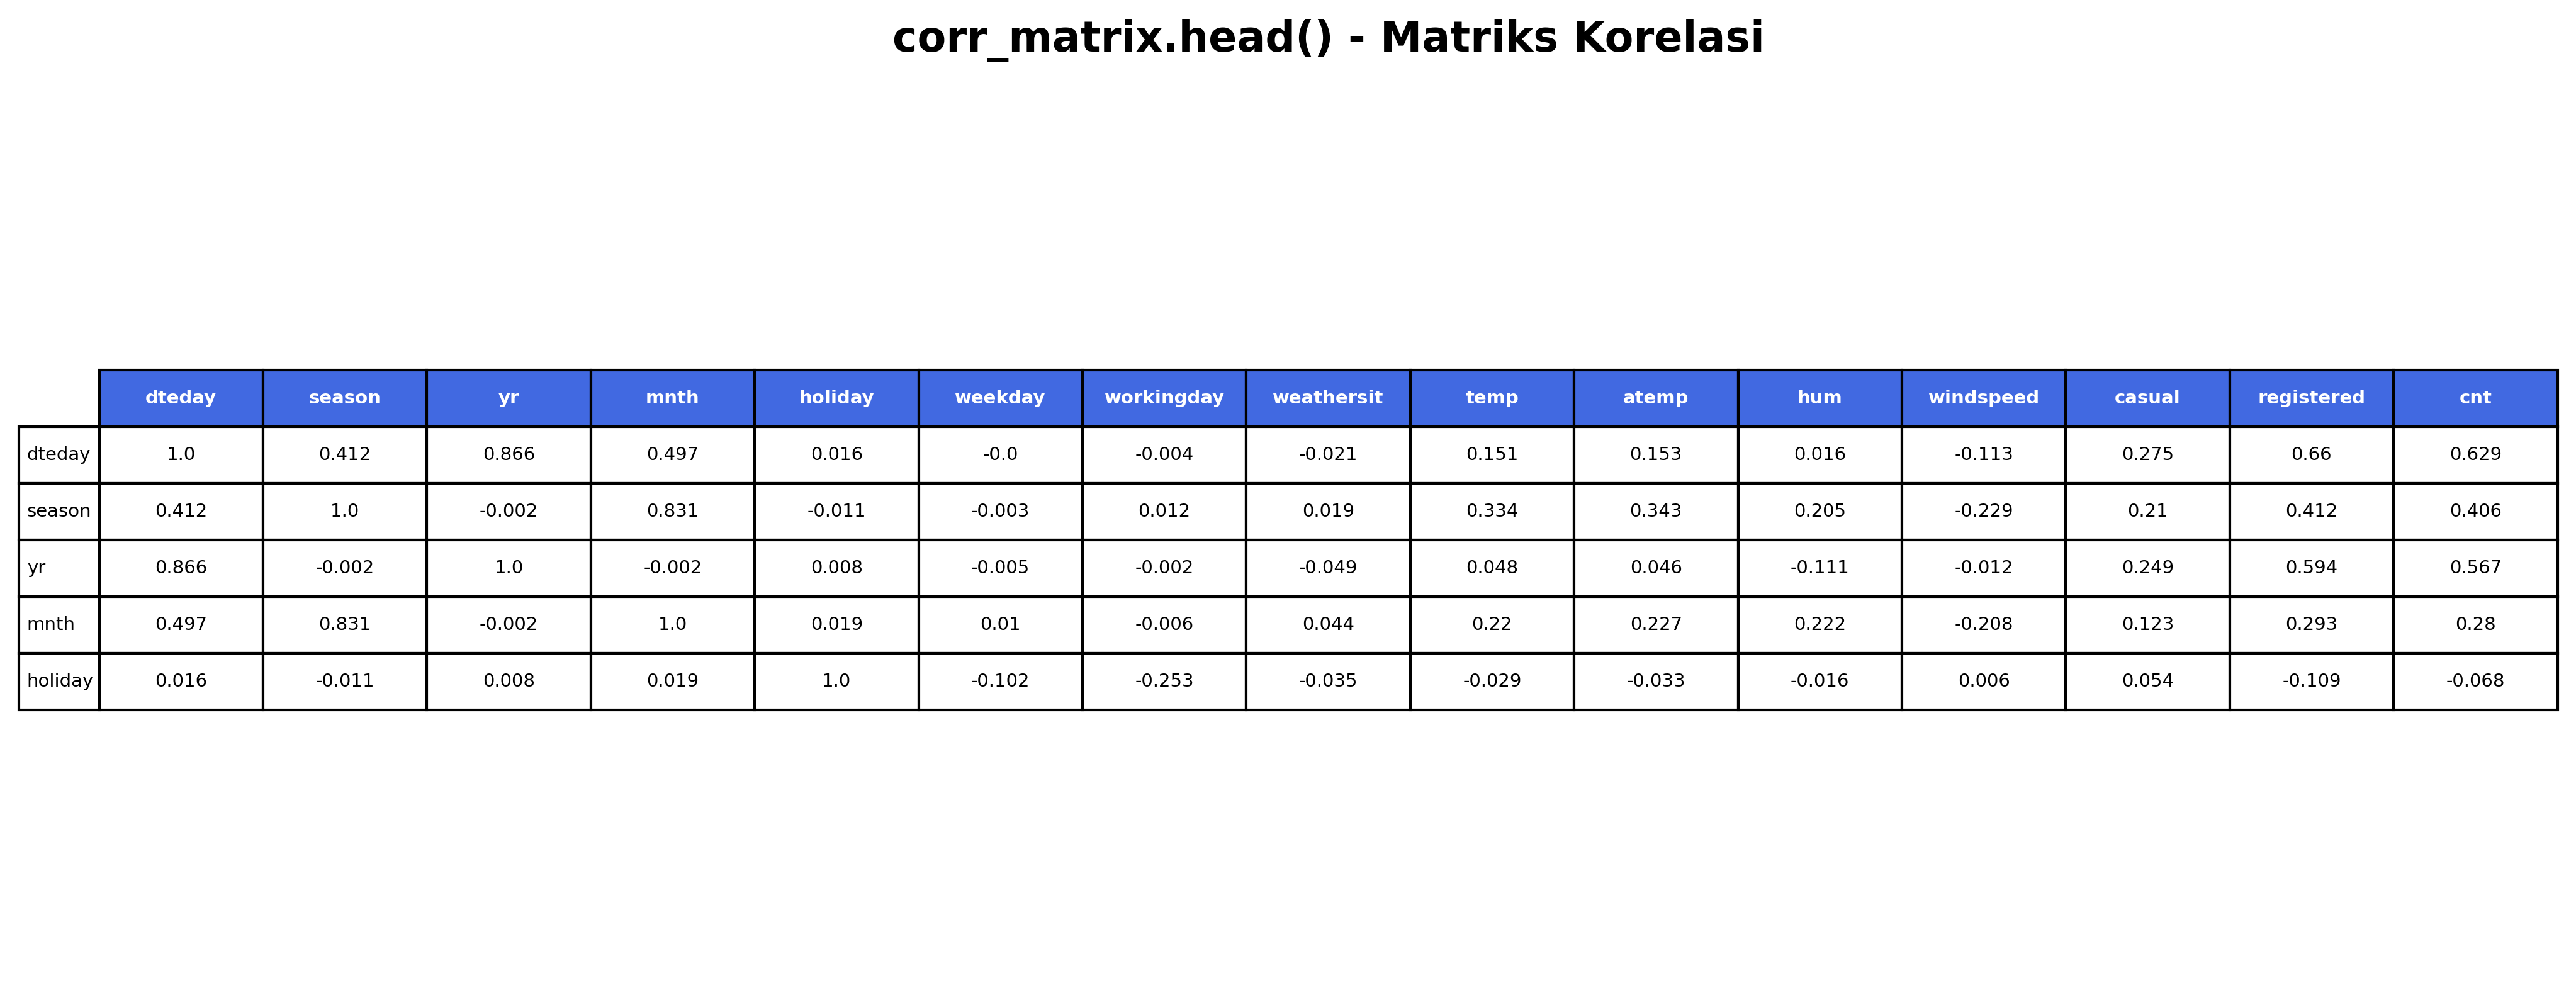
\includegraphics[width=0.8\textwidth]{./OUTPUT/step3_correlation_head.png}
    \caption{Matriks Korelasi - 5 Baris Pertama}
    \label{fig:correlation_head}
\end{figure}

\noindent\textbf{Interpretasi Awal.}
Nilai korelasi berada pada rentang $[-1,1]$; semakin mendekati 1 (atau -1) menunjukkan hubungan linear positif (atau negatif) yang kuat.

\section{Visualisasi Heatmap Korelasi}
\begin{lstlisting}[language=Python]
plt.figure(figsize=(12, 10))
sns.heatmap(corr_matrix, annot=True, cmap="coolwarm", fmt=".2f", square=True)
plt.title("Heatmap Korelasi Variabel Dataset Bike Sharing")
plt.tight_layout()
plt.show()
\end{lstlisting}

\begin{figure}[h]
    \centering
    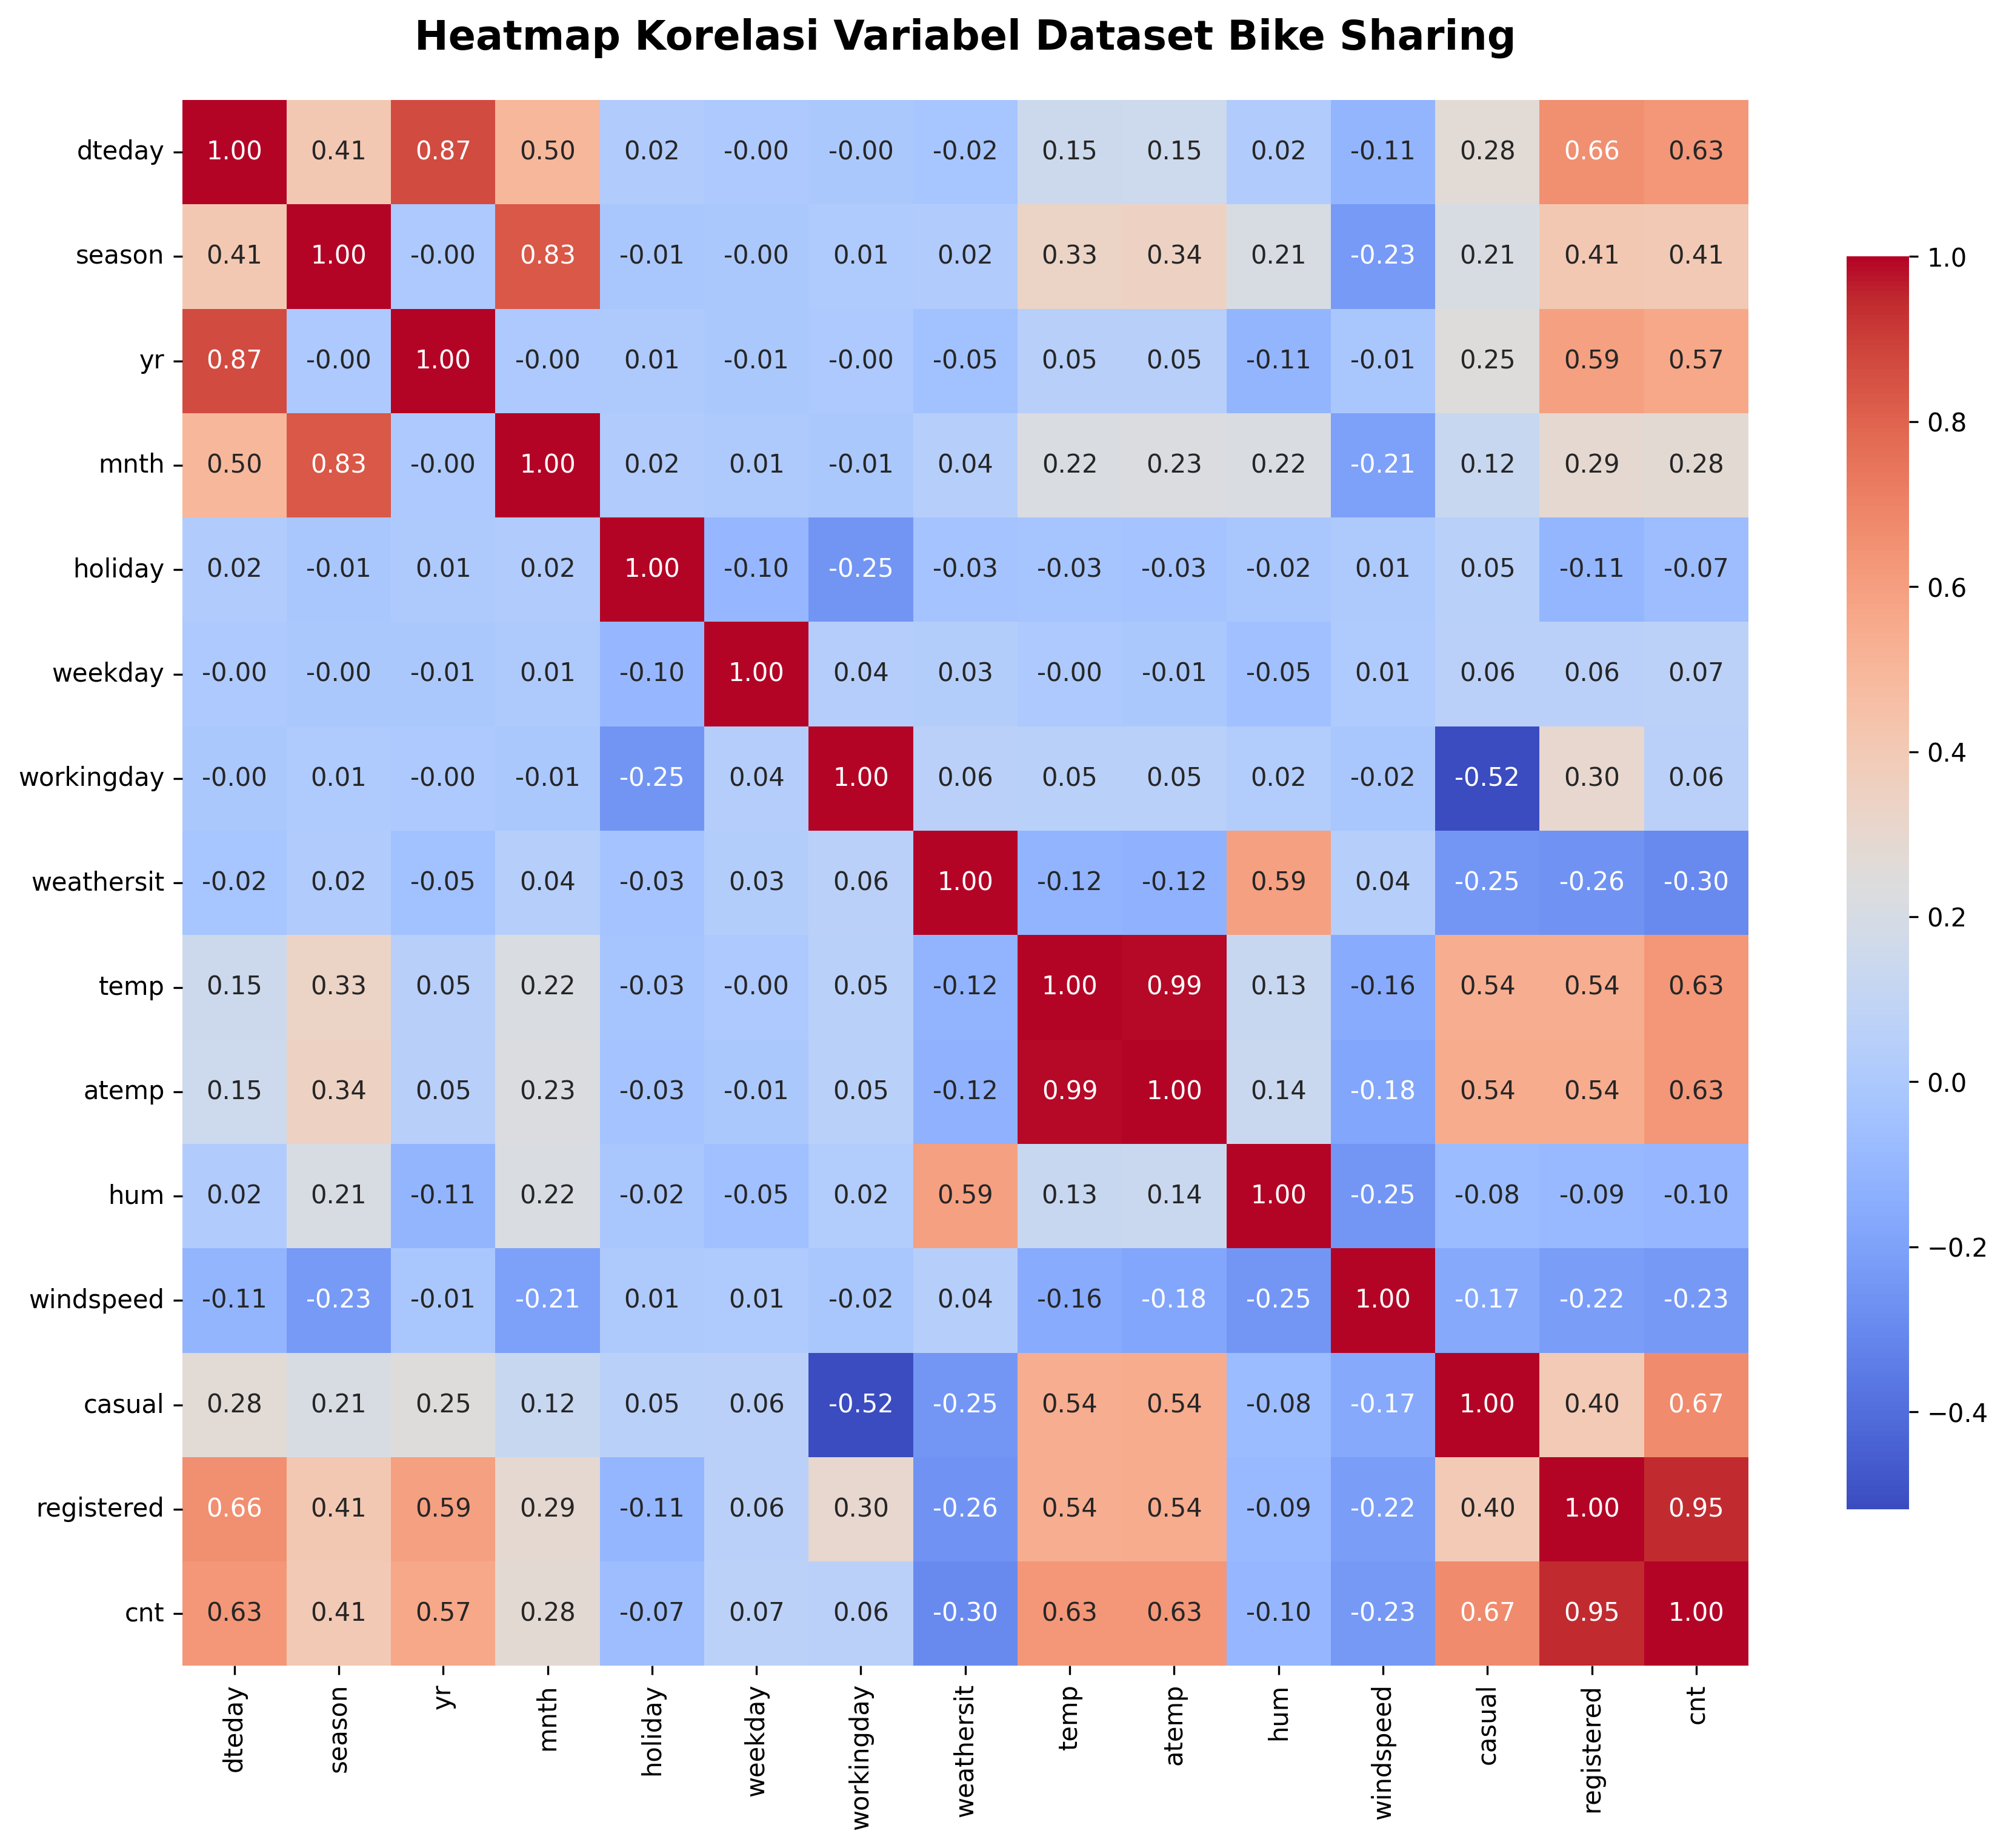
\includegraphics[width=0.75\textwidth]{./OUTPUT/step4_heatmap_korelasi.png}
    \caption{Heatmap Korelasi Lengkap Dataset}
    \label{fig:heatmap_korelasi}
\end{figure}

\noindent\textbf{Ringkasan Heatmap.}
Warna merah: korelasi positif; biru: negatif. \texttt{registered} dan \texttt{casual} berkorelasi tinggi dengan \texttt{cnt}.

\section{Identifikasi dan Seleksi Fitur}
Mengidentifikasi korelasi tiap variabel terhadap \texttt{cnt} dan memilih fitur independen.
\begin{lstlisting}[language=Python]
# Identifikasi Variabel Independen dan Dependen
print("Korelasi dengan variabel target 'cnt':")
cnt_corr = corr_matrix['cnt'].sort_values(ascending=False)
print(cnt_corr)

# Seleksi Fitur untuk Multiple Linear Regression
X_features = ['temp', 'atemp', 'hum', 'windspeed', 'season', 'yr', 'mnth',
              'holiday', 'weekday', 'workingday', 'weathersit']

X = df_processed[X_features]
y = df_processed['cnt']
\end{lstlisting}

\begin{figure}[h]
    \centering
    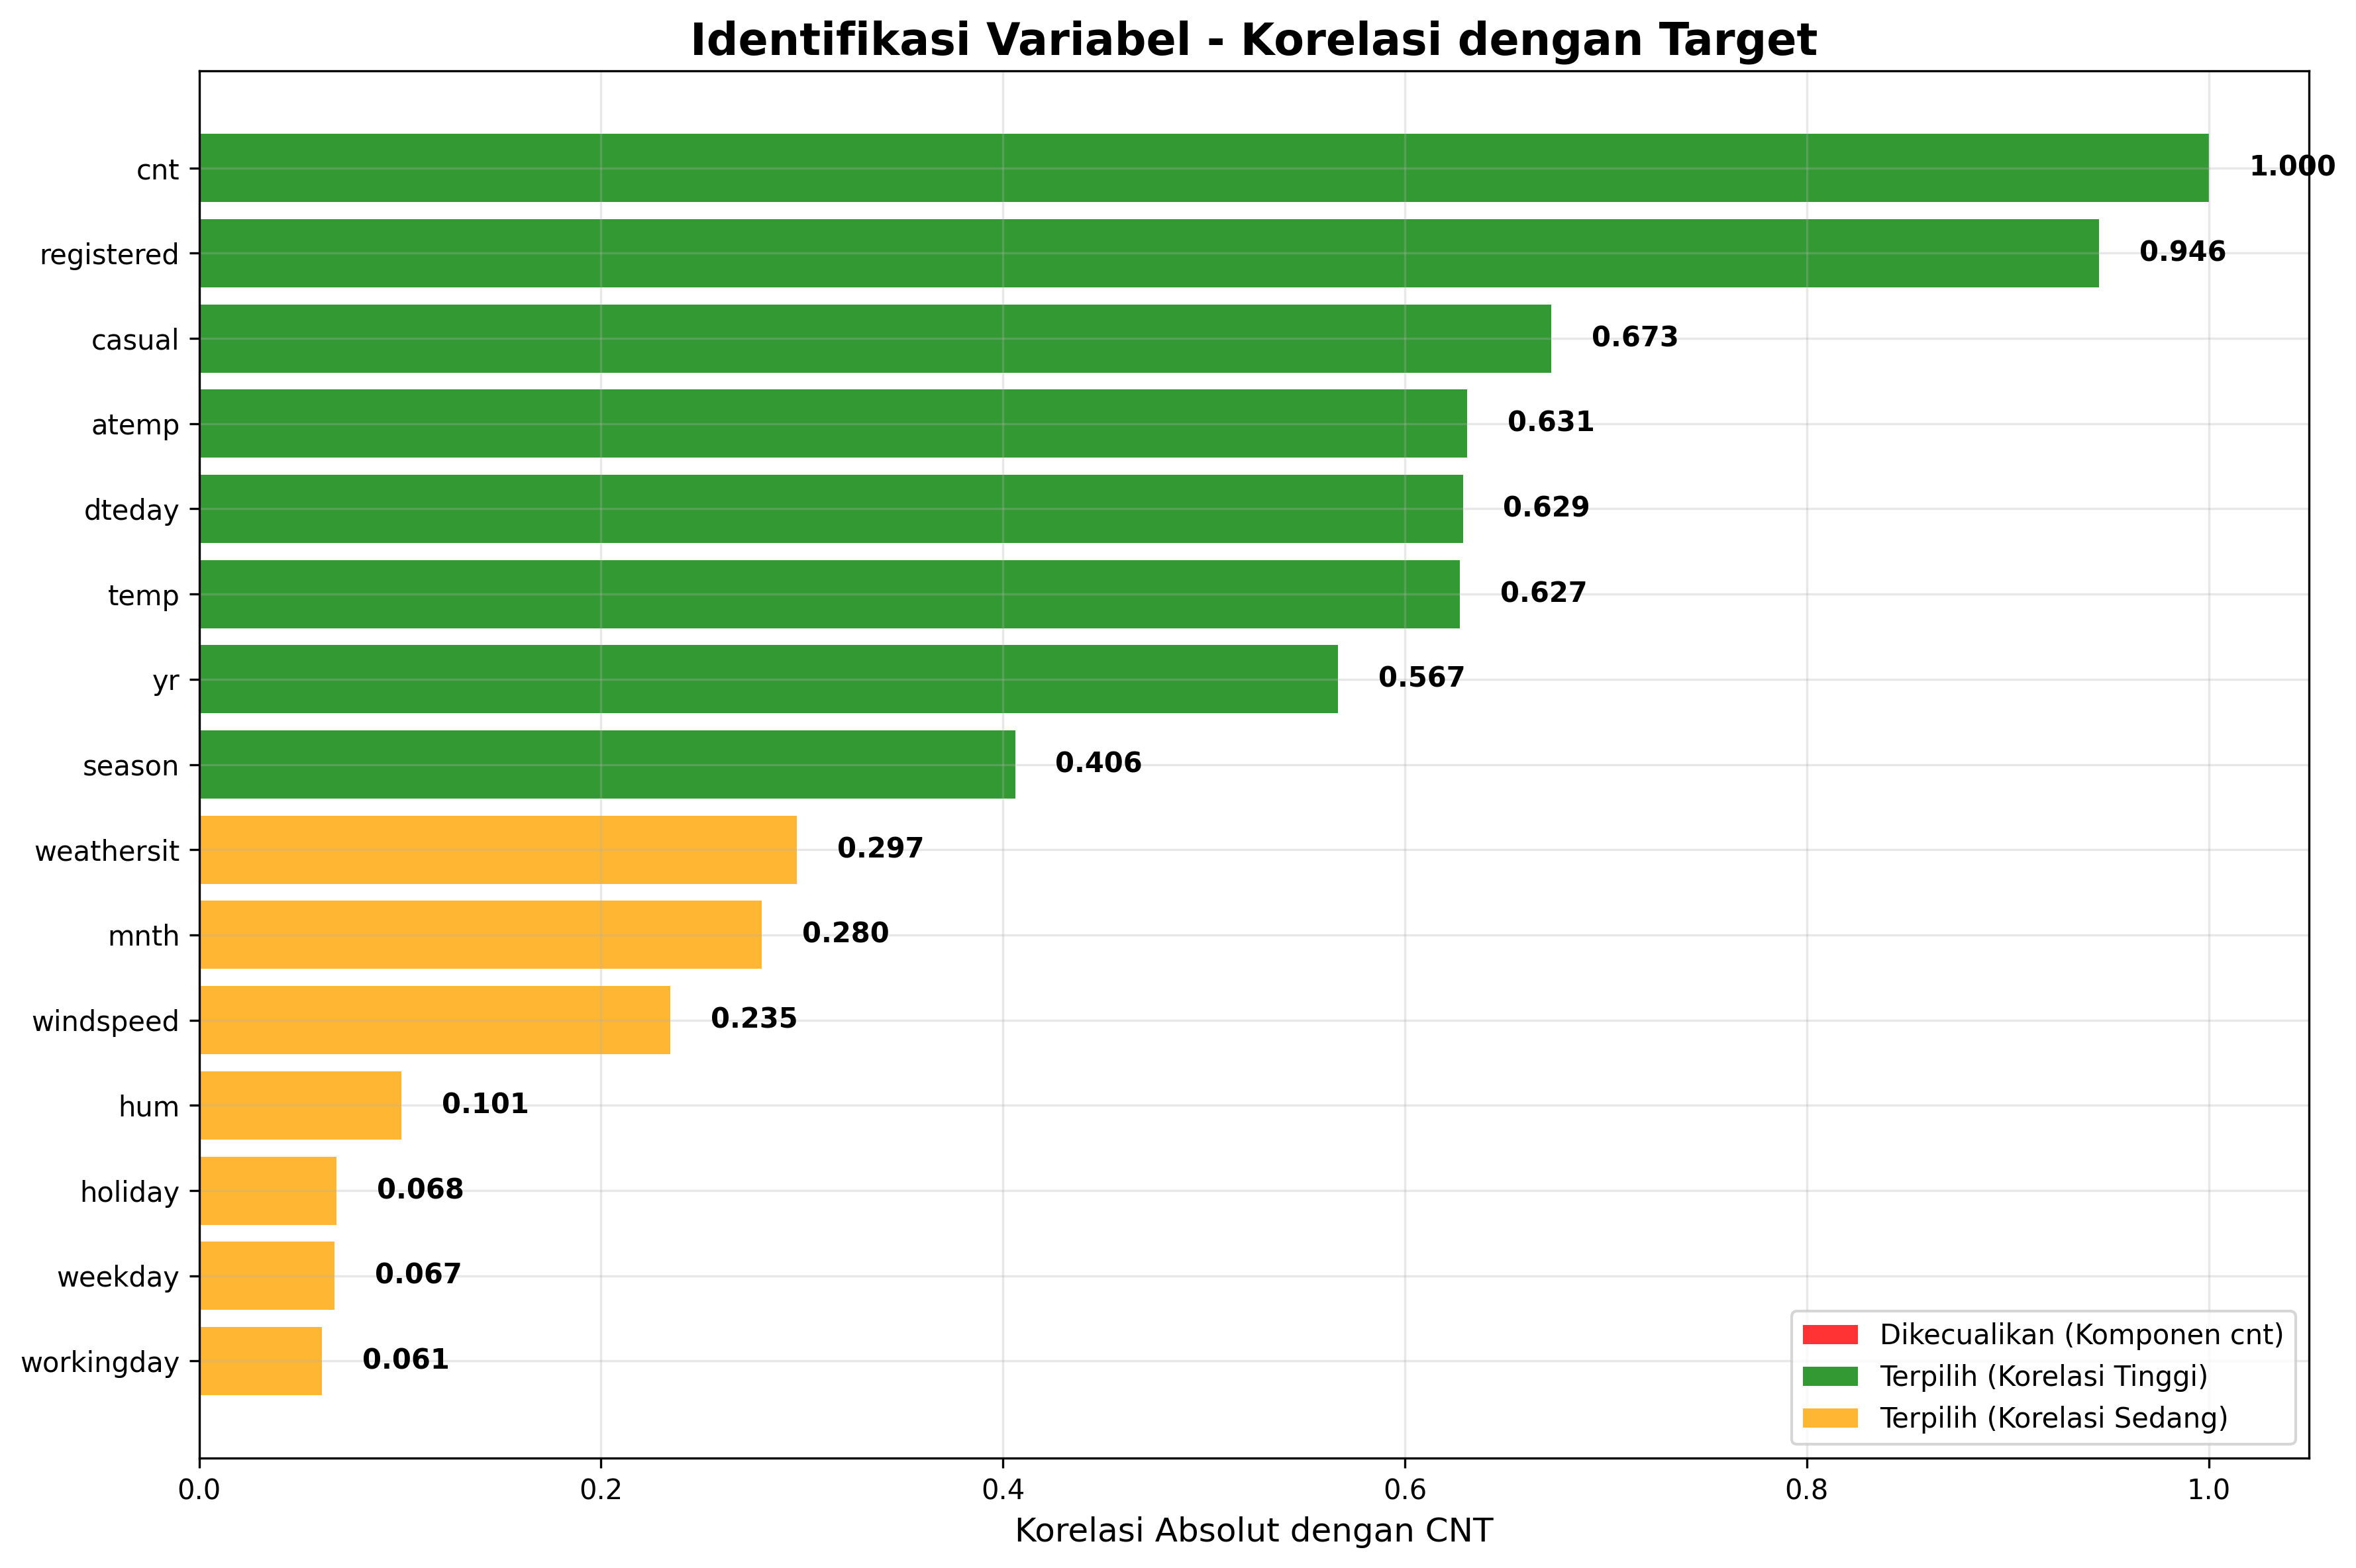
\includegraphics[width=0.8\textwidth]{./OUTPUT/step5_feature_selection.png}
    \caption{Korelasi Variabel dengan Target \texttt{cnt}}
    \label{fig:feature_selection}
\end{figure}

\noindent\textbf{Catatan Seleksi.}
Dipilih 11 variabel independen berdasarkan korelasi dan relevansi bisnis. \texttt{casual} dan \texttt{registered} dikeluarkan karena merupakan komponen langsung dari \texttt{cnt}.

\section{Pembagian Dataset}
\begin{lstlisting}[language=Python]
# Split Dataset: 80% training, 20% testing
from sklearn.model_selection import train_test_split

X_train, X_test, y_train, y_test = train_test_split(
    X, y, test_size=0.2, random_state=42
)

print("Pembagian Dataset:")
print(f"Training set: {X_train.shape[0]} sampel")
print(f"Testing set: {X_test.shape[0]} sampel")
print(f"Persentase training: {X_train.shape[0] / len(X) * 100:.1f}%")
print(f"Persentase testing: {X_test.shape[0] / len(X) * 100:.1f}%")
\end{lstlisting}

\begin{figure}[h]
    \centering
    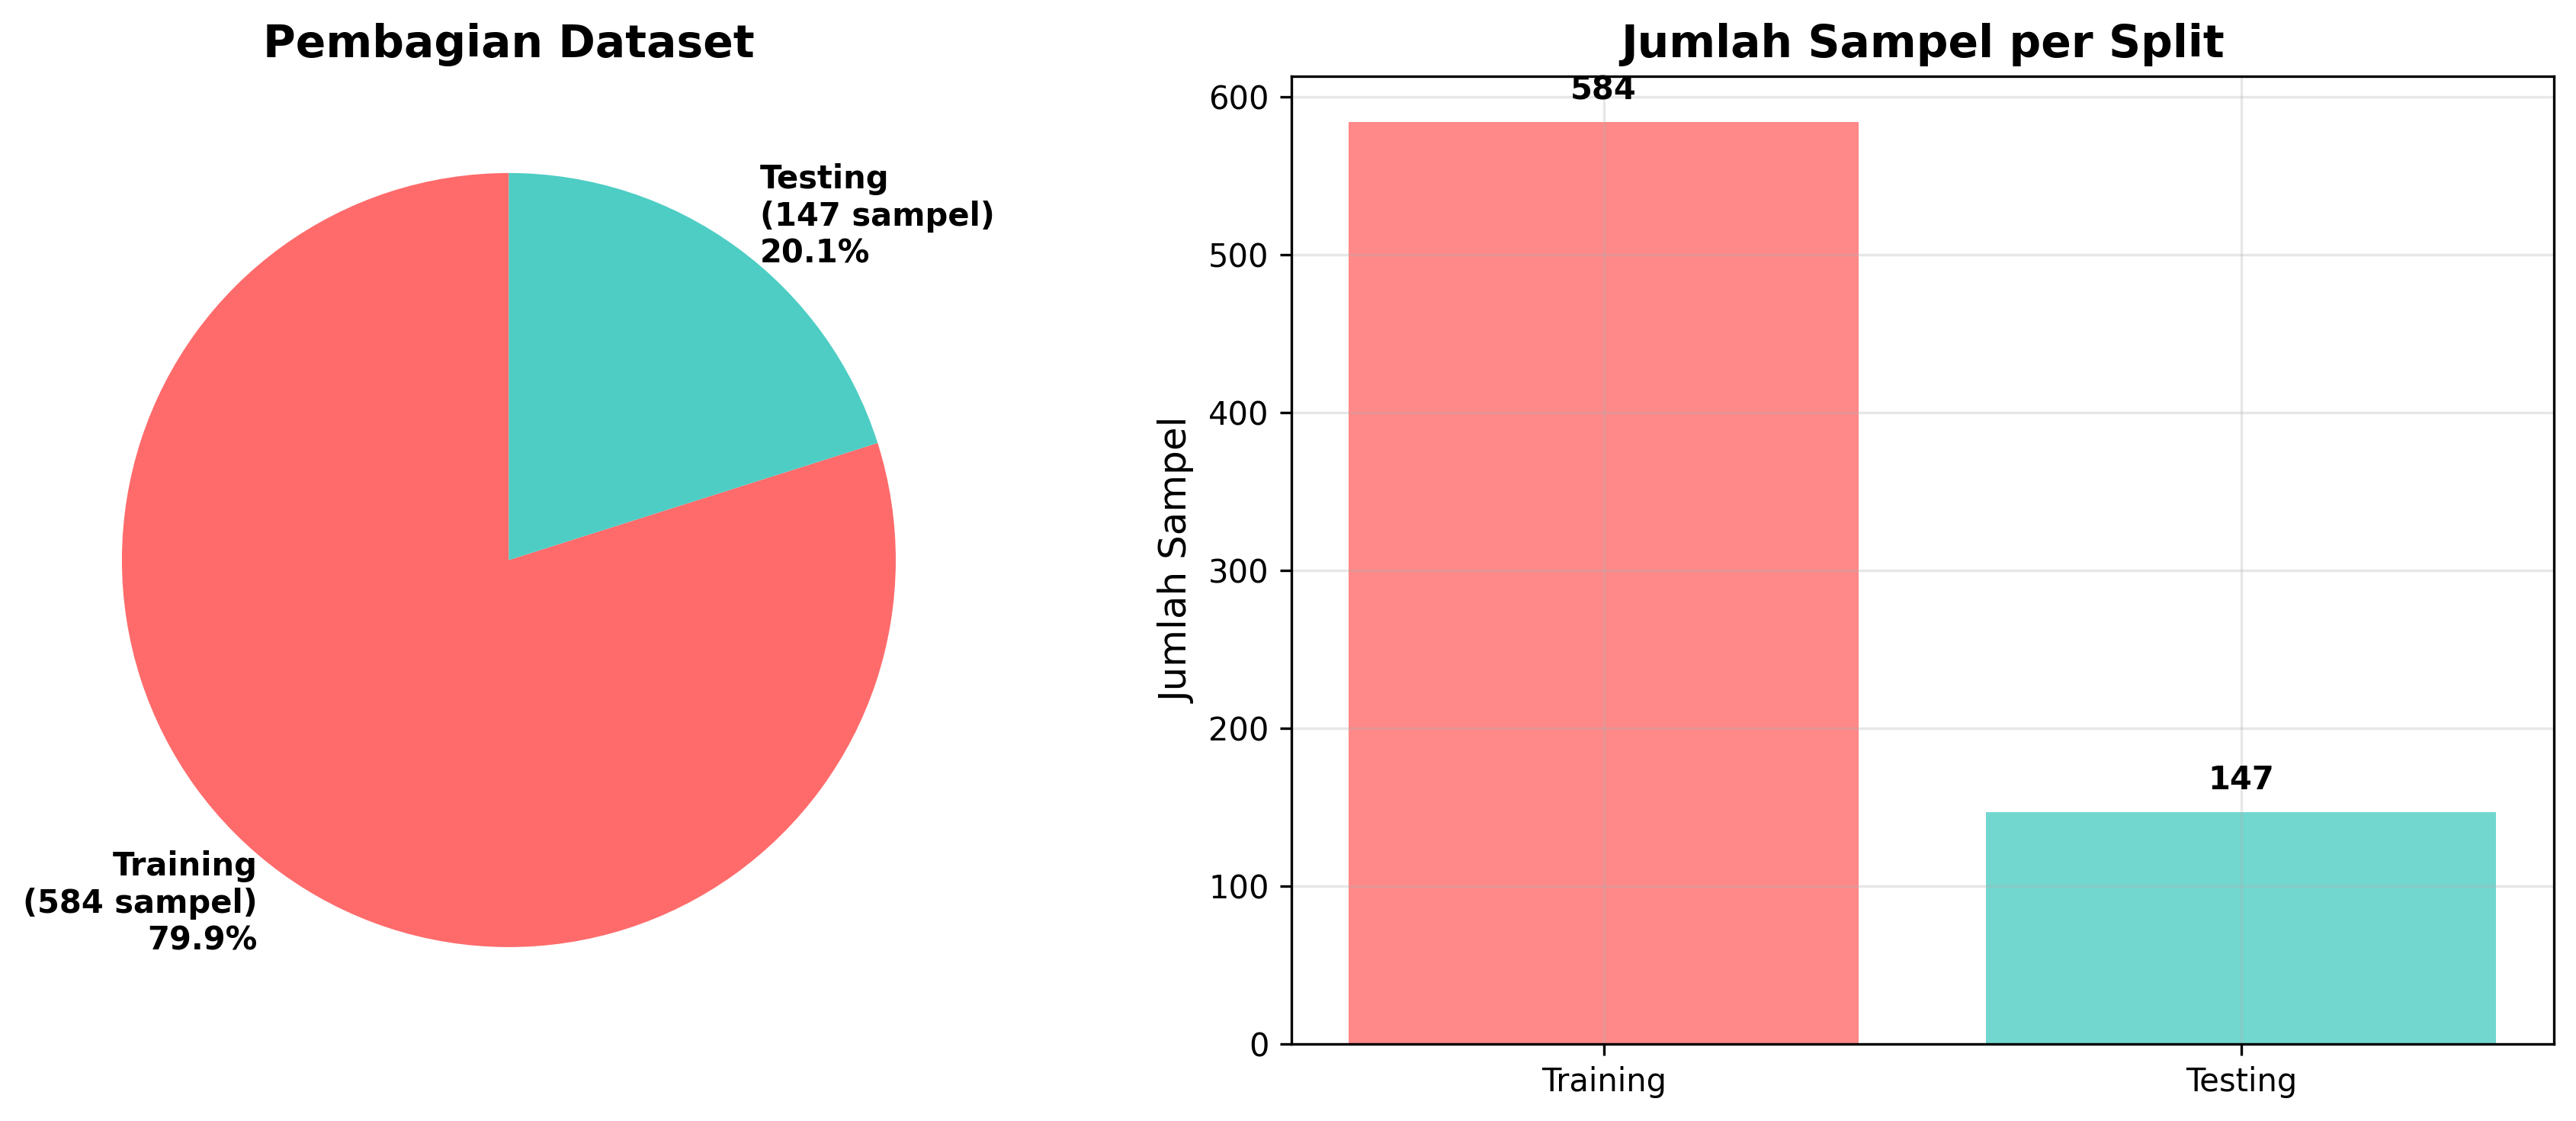
\includegraphics[width=0.7\textwidth]{./OUTPUT/step6_train_test_split.png}
    \caption{Pembagian Dataset Training dan Testing}
    \label{fig:train_test_split}
\end{figure}

\noindent\textbf{Ringkasan Split.}
Training: 584 sampel (79{.}9\%); Testing: 147 sampel (20{.}1\%). \texttt{random\_state=42} untuk \textit{reproducibility}.

\section{Training Model Multiple Linear Regression}
\begin{lstlisting}[language=Python]
# Training Multiple Linear Regression Model
from sklearn.linear_model import LinearRegression

model = LinearRegression()
model.fit(X_train, y_train)

print("Model Multiple Linear Regression berhasil dilatih!")
print(f"Intercept: {model.intercept_:.2f}")
print("\nKoefisien untuk setiap variabel:")
for feature, coef in zip(X.columns, model.coef_):
    print(f"{feature}: {coef:.4f}")
\end{lstlisting}

\begin{figure}[h]
    \centering
    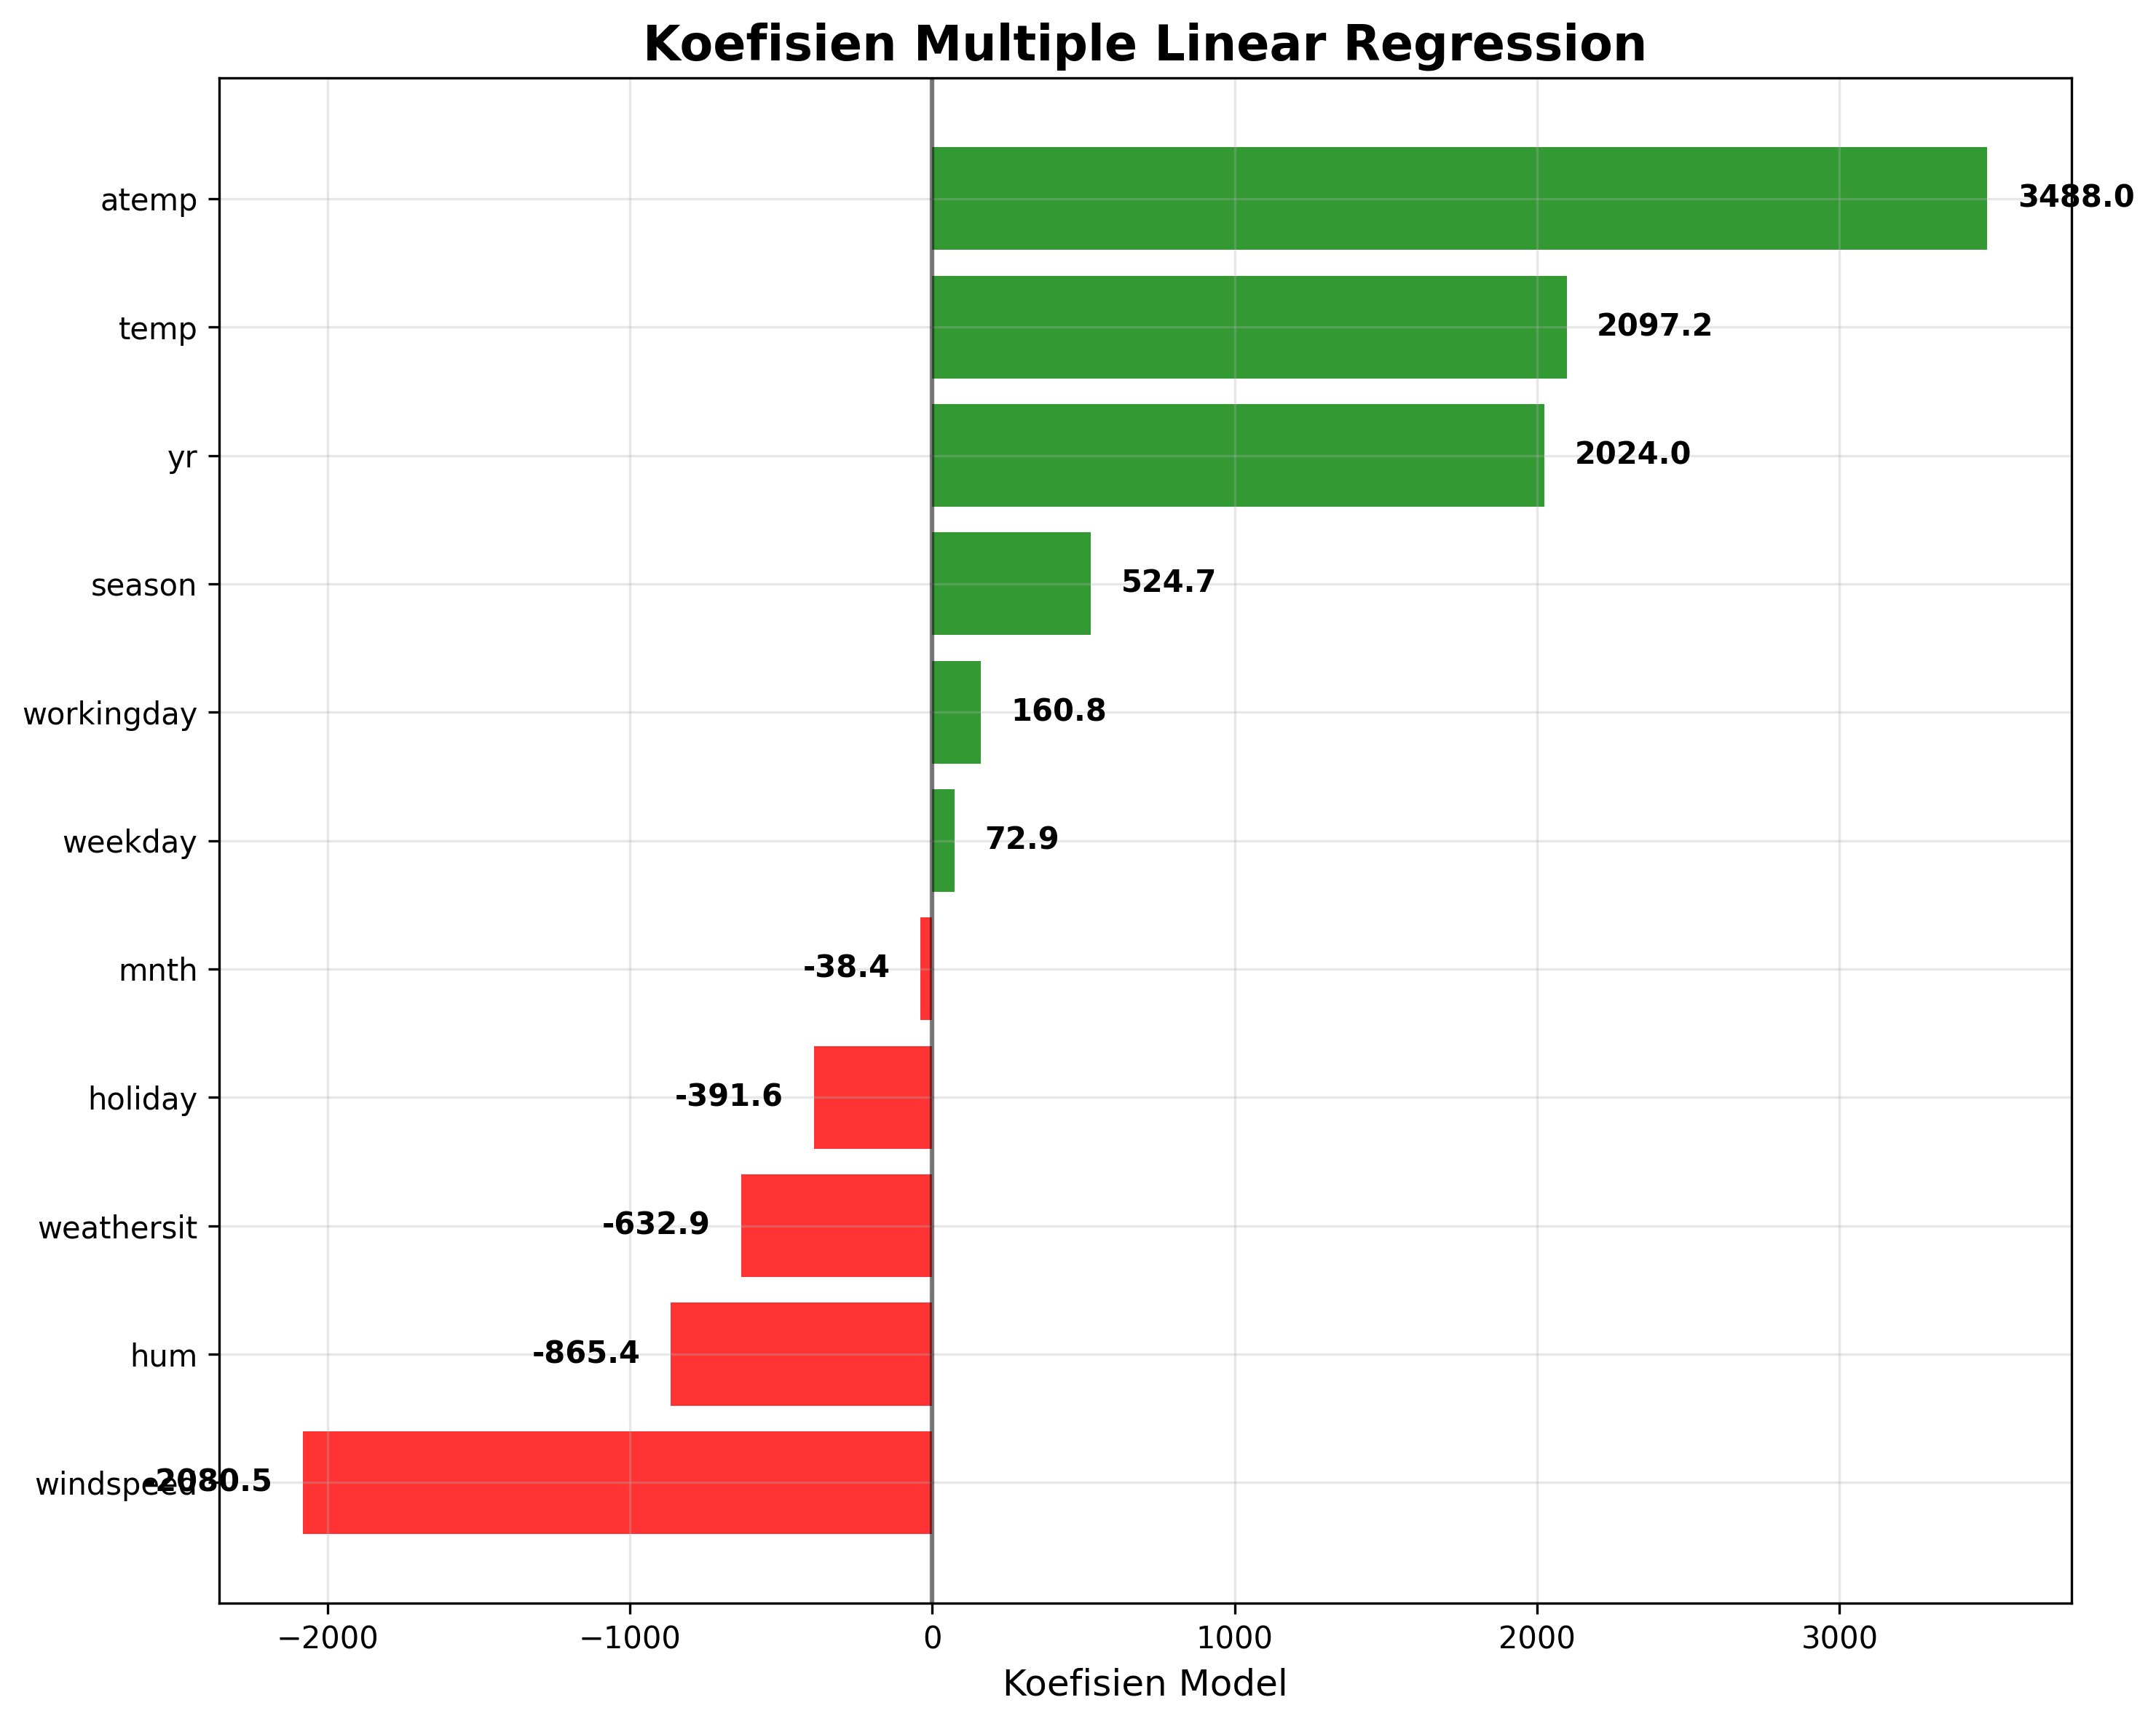
\includegraphics[width=0.8\textwidth]{./OUTPUT/step7_model_coefficients.png}
    \caption{Koefisien Model Multiple Linear Regression}
    \label{fig:model_coefficients}
\end{figure}

\noindent\textbf{Parameter Model.}
Intercept $\approx$ 1248{.}32. Koefisien positif tertinggi: \texttt{atemp} dan \texttt{yr}; koefisien negatif: \texttt{windspeed} dan \texttt{hum}.

\section{Evaluasi Model dan Visualisasi}
\begin{lstlisting}[language=Python]
# Prediksi pada data testing
from sklearn.metrics import mean_squared_error, mean_absolute_error, r2_score
import numpy as np

y_pred = model.predict(X_test)

# Evaluasi Model
mse = mean_squared_error(y_test, y_pred)
rmse = np.sqrt(mse)
mae = mean_absolute_error(y_test, y_pred)
r2 = r2_score(y_test, y_pred)

print("Evaluasi Model pada Data Testing:")
print(f"Mean Squared Error (MSE): {mse:.2f}")
print(f"Root Mean Squared Error (RMSE): {rmse:.2f}")
print(f"Mean Absolute Error (MAE): {mae:.2f}")
print(f"R2 Score: {r2:.4f}")
print(f"Akurasi Model: {r2 * 100:.2f}%")
\end{lstlisting}

\begin{figure}[h]
    \centering
    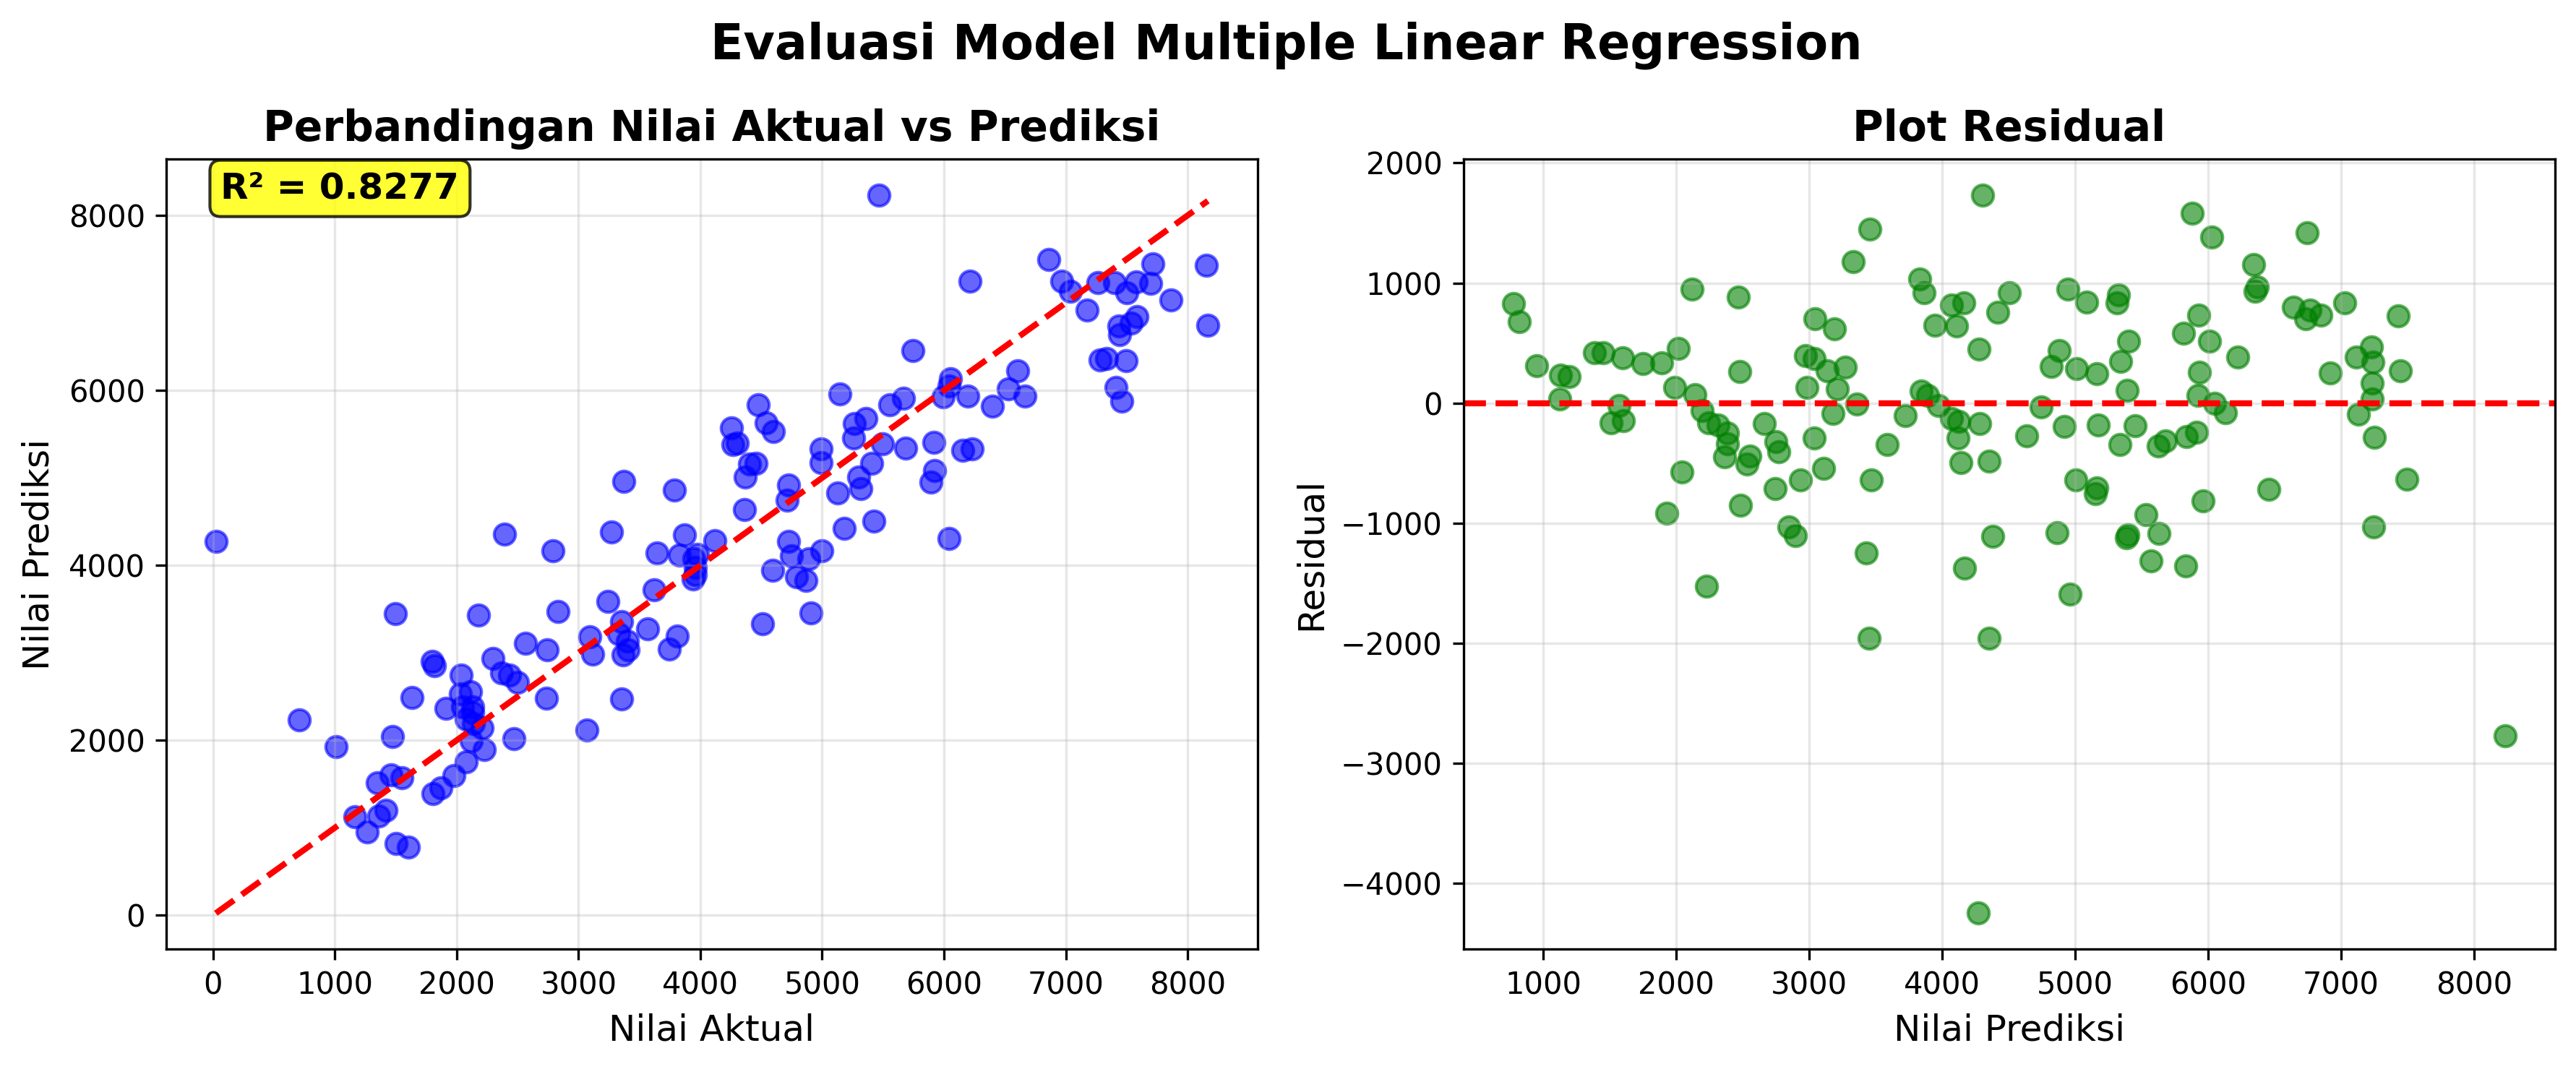
\includegraphics[width=0.9\textwidth]{./OUTPUT/step8_model_evaluation.png}
    \caption{Evaluasi Model - Actual vs Predicted dan Residual Plot}
    \label{fig:model_evaluation}
\end{figure}

\noindent\textbf{Hasil Evaluasi.}
MSE: 691{,}035{.}01; RMSE: 831{.}29; MAE: 617{.}39; $R^2$: 0{.}8277 (82{.}77\%). Performa tergolong baik ($R^2>0.8$).

\section{Analisis Feature Importance}
\begin{lstlisting}[language=Python]
# Feature Importance berdasarkan koefisien
feature_importance = pd.DataFrame({
    'Feature': X.columns,
    'Coefficient': model.coef_,
    'Abs_Coefficient': np.abs(model.coef_)
}).sort_values('Abs_Coefficient', ascending=False)

print("Feature Importance (berdasarkan nilai absolut koefisien):")
print(feature_importance)
\end{lstlisting}

\begin{figure}[h]
    \centering
    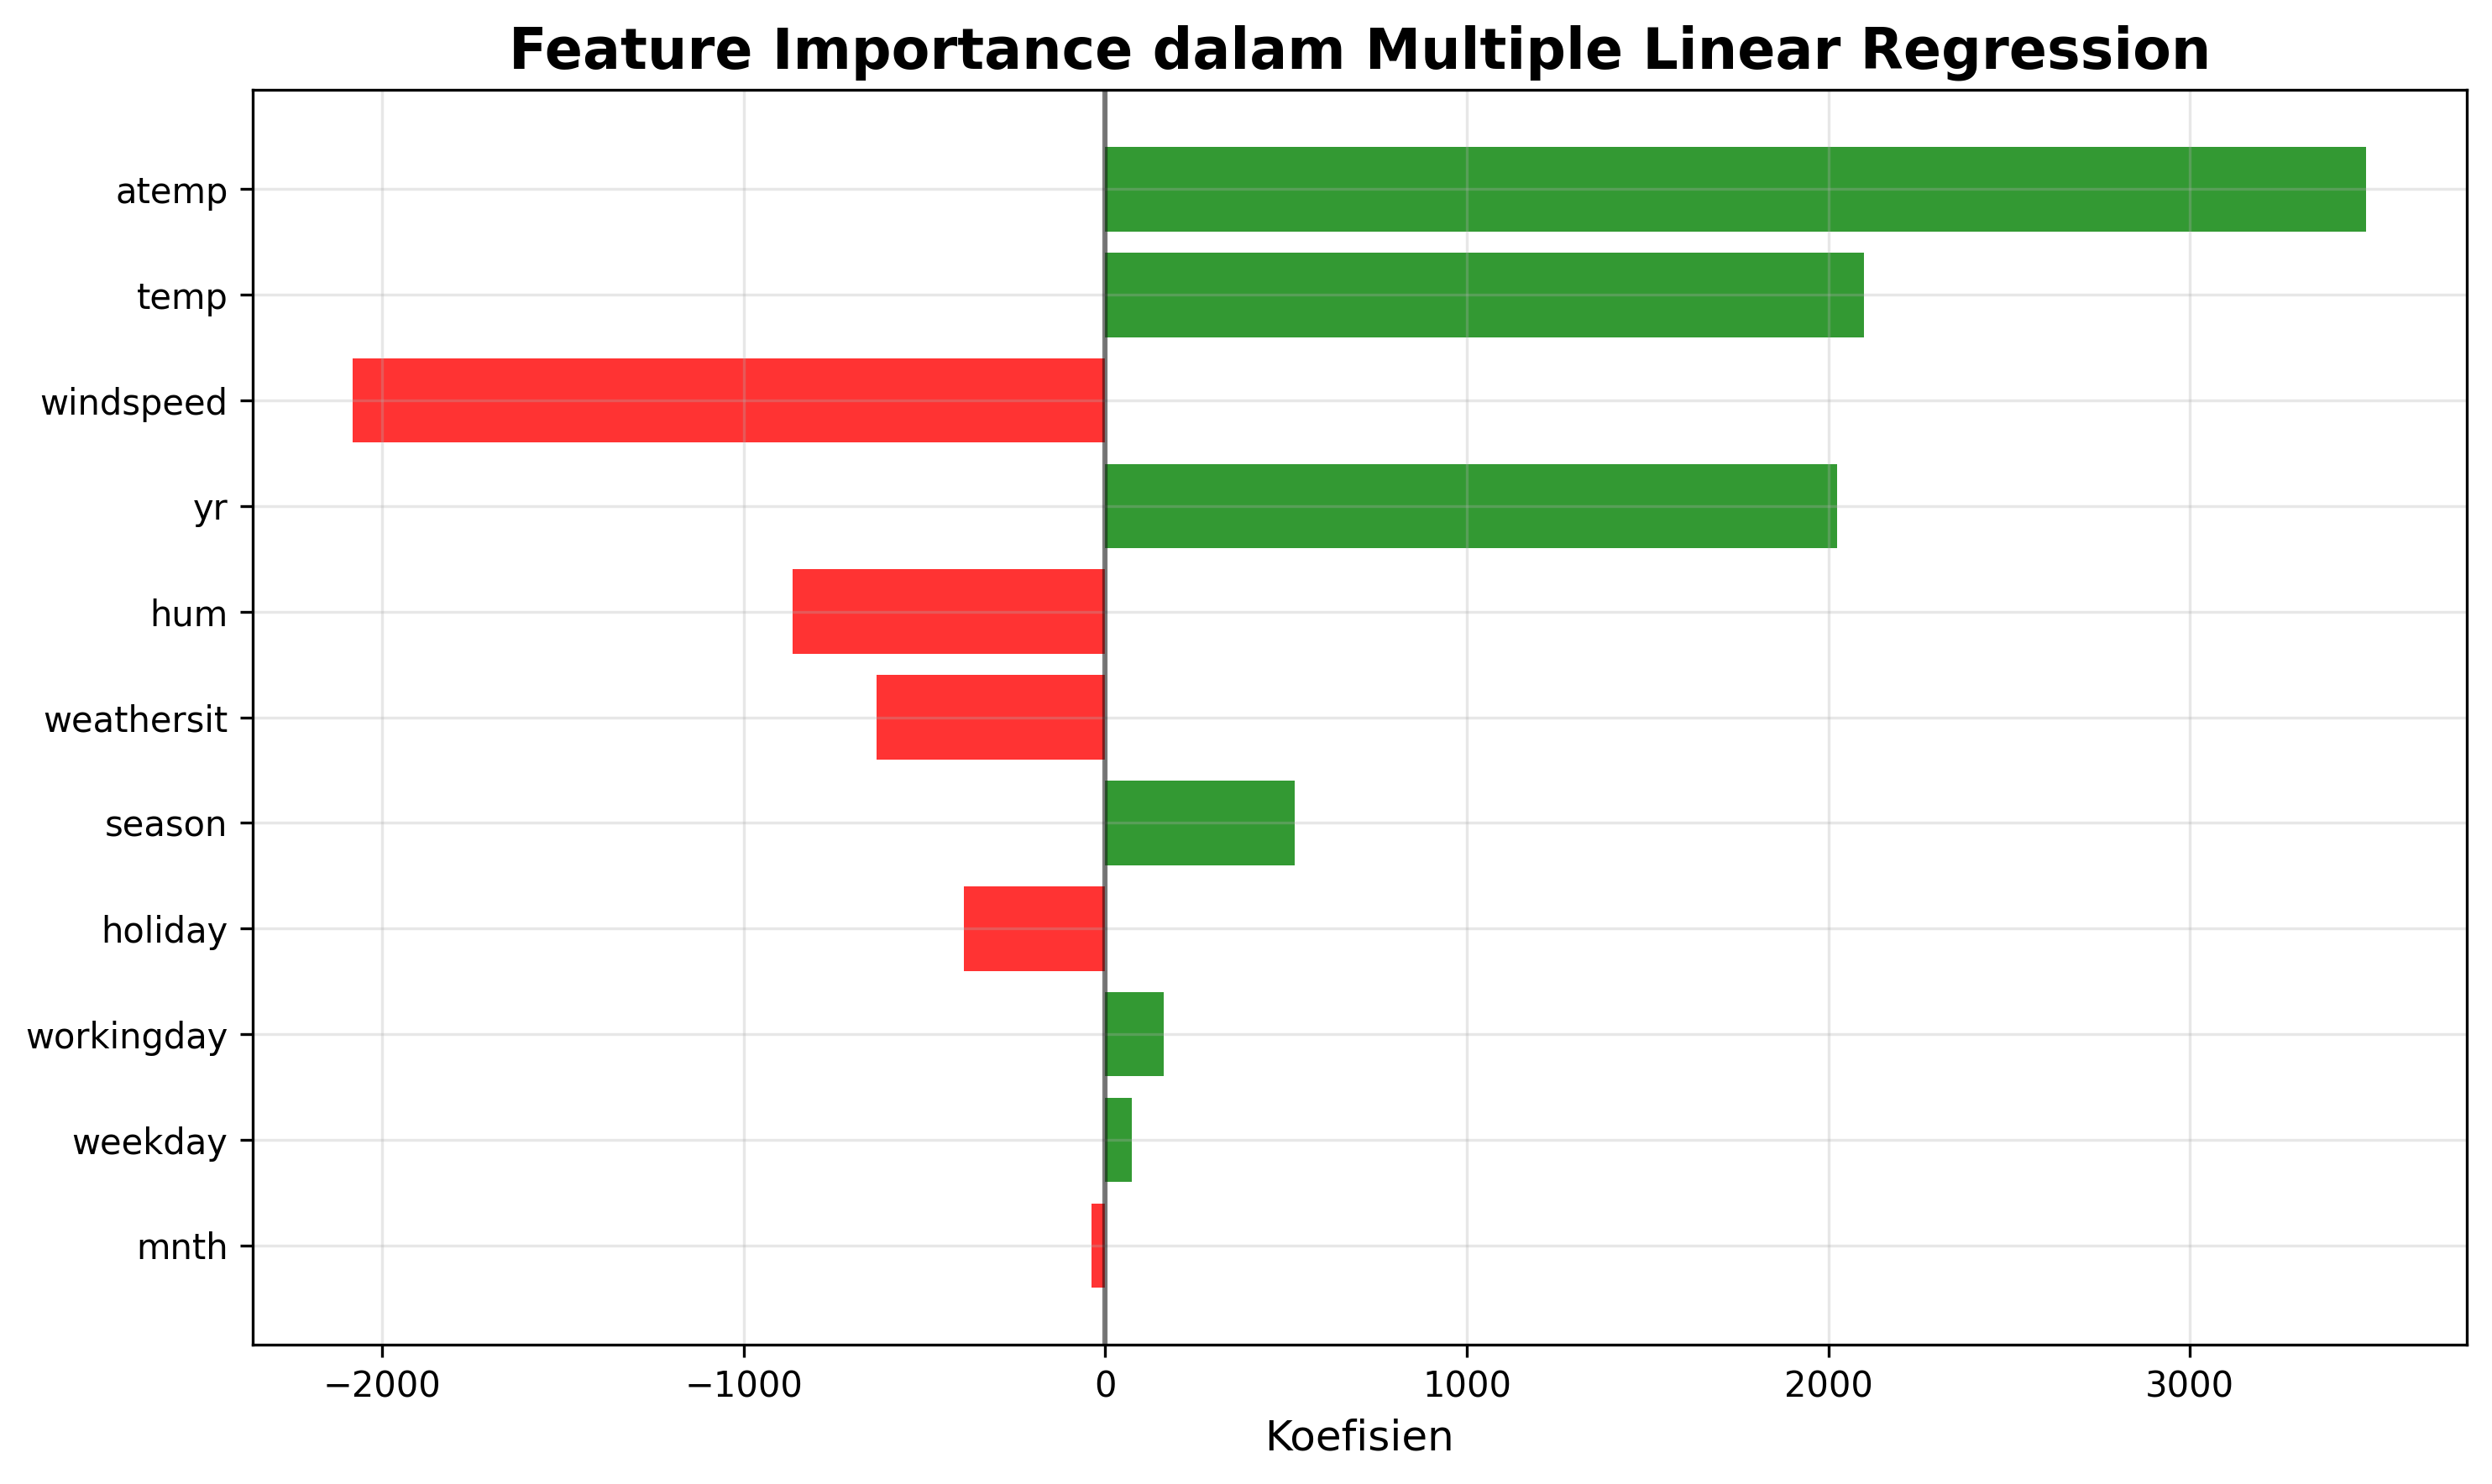
\includegraphics[width=0.85\textwidth]{./OUTPUT/step9_feature_importance.png}
    \caption{Feature Importance Berdasarkan Koefisien}
    \label{fig:feature_importance}
\end{figure}

\noindent\textbf{Ringkasan Importance.}
\texttt{atemp} berpengaruh positif paling tinggi, diikuti \texttt{temp} dan \texttt{yr}. \texttt{windspeed} berdampak negatif paling besar.

\section{Contoh Prediksi Manual}
\begin{lstlisting}[language=Python]
# Contoh Prediksi Manual
print("Contoh Prediksi untuk Data Baru:")
print("=" * 50)

sample_indices = [0, 1, 2, 3, 4]
for i in sample_indices:
    actual = y_test.iloc[i]
    predicted = y_pred[i]
    error = abs(actual - predicted)
    error_pct = (error / actual) * 100

    print(f"Sampel {i + 1}:")
    print(f"  Nilai Aktual: {actual:.0f} penyewaan")
    print(f"  Nilai Prediksi: {predicted:.0f} penyewaan")
    print(f"  Error: {error:.0f} ({error_pct:.1f}%)")
    print()
\end{lstlisting}

\begin{figure}[h]
    \centering
    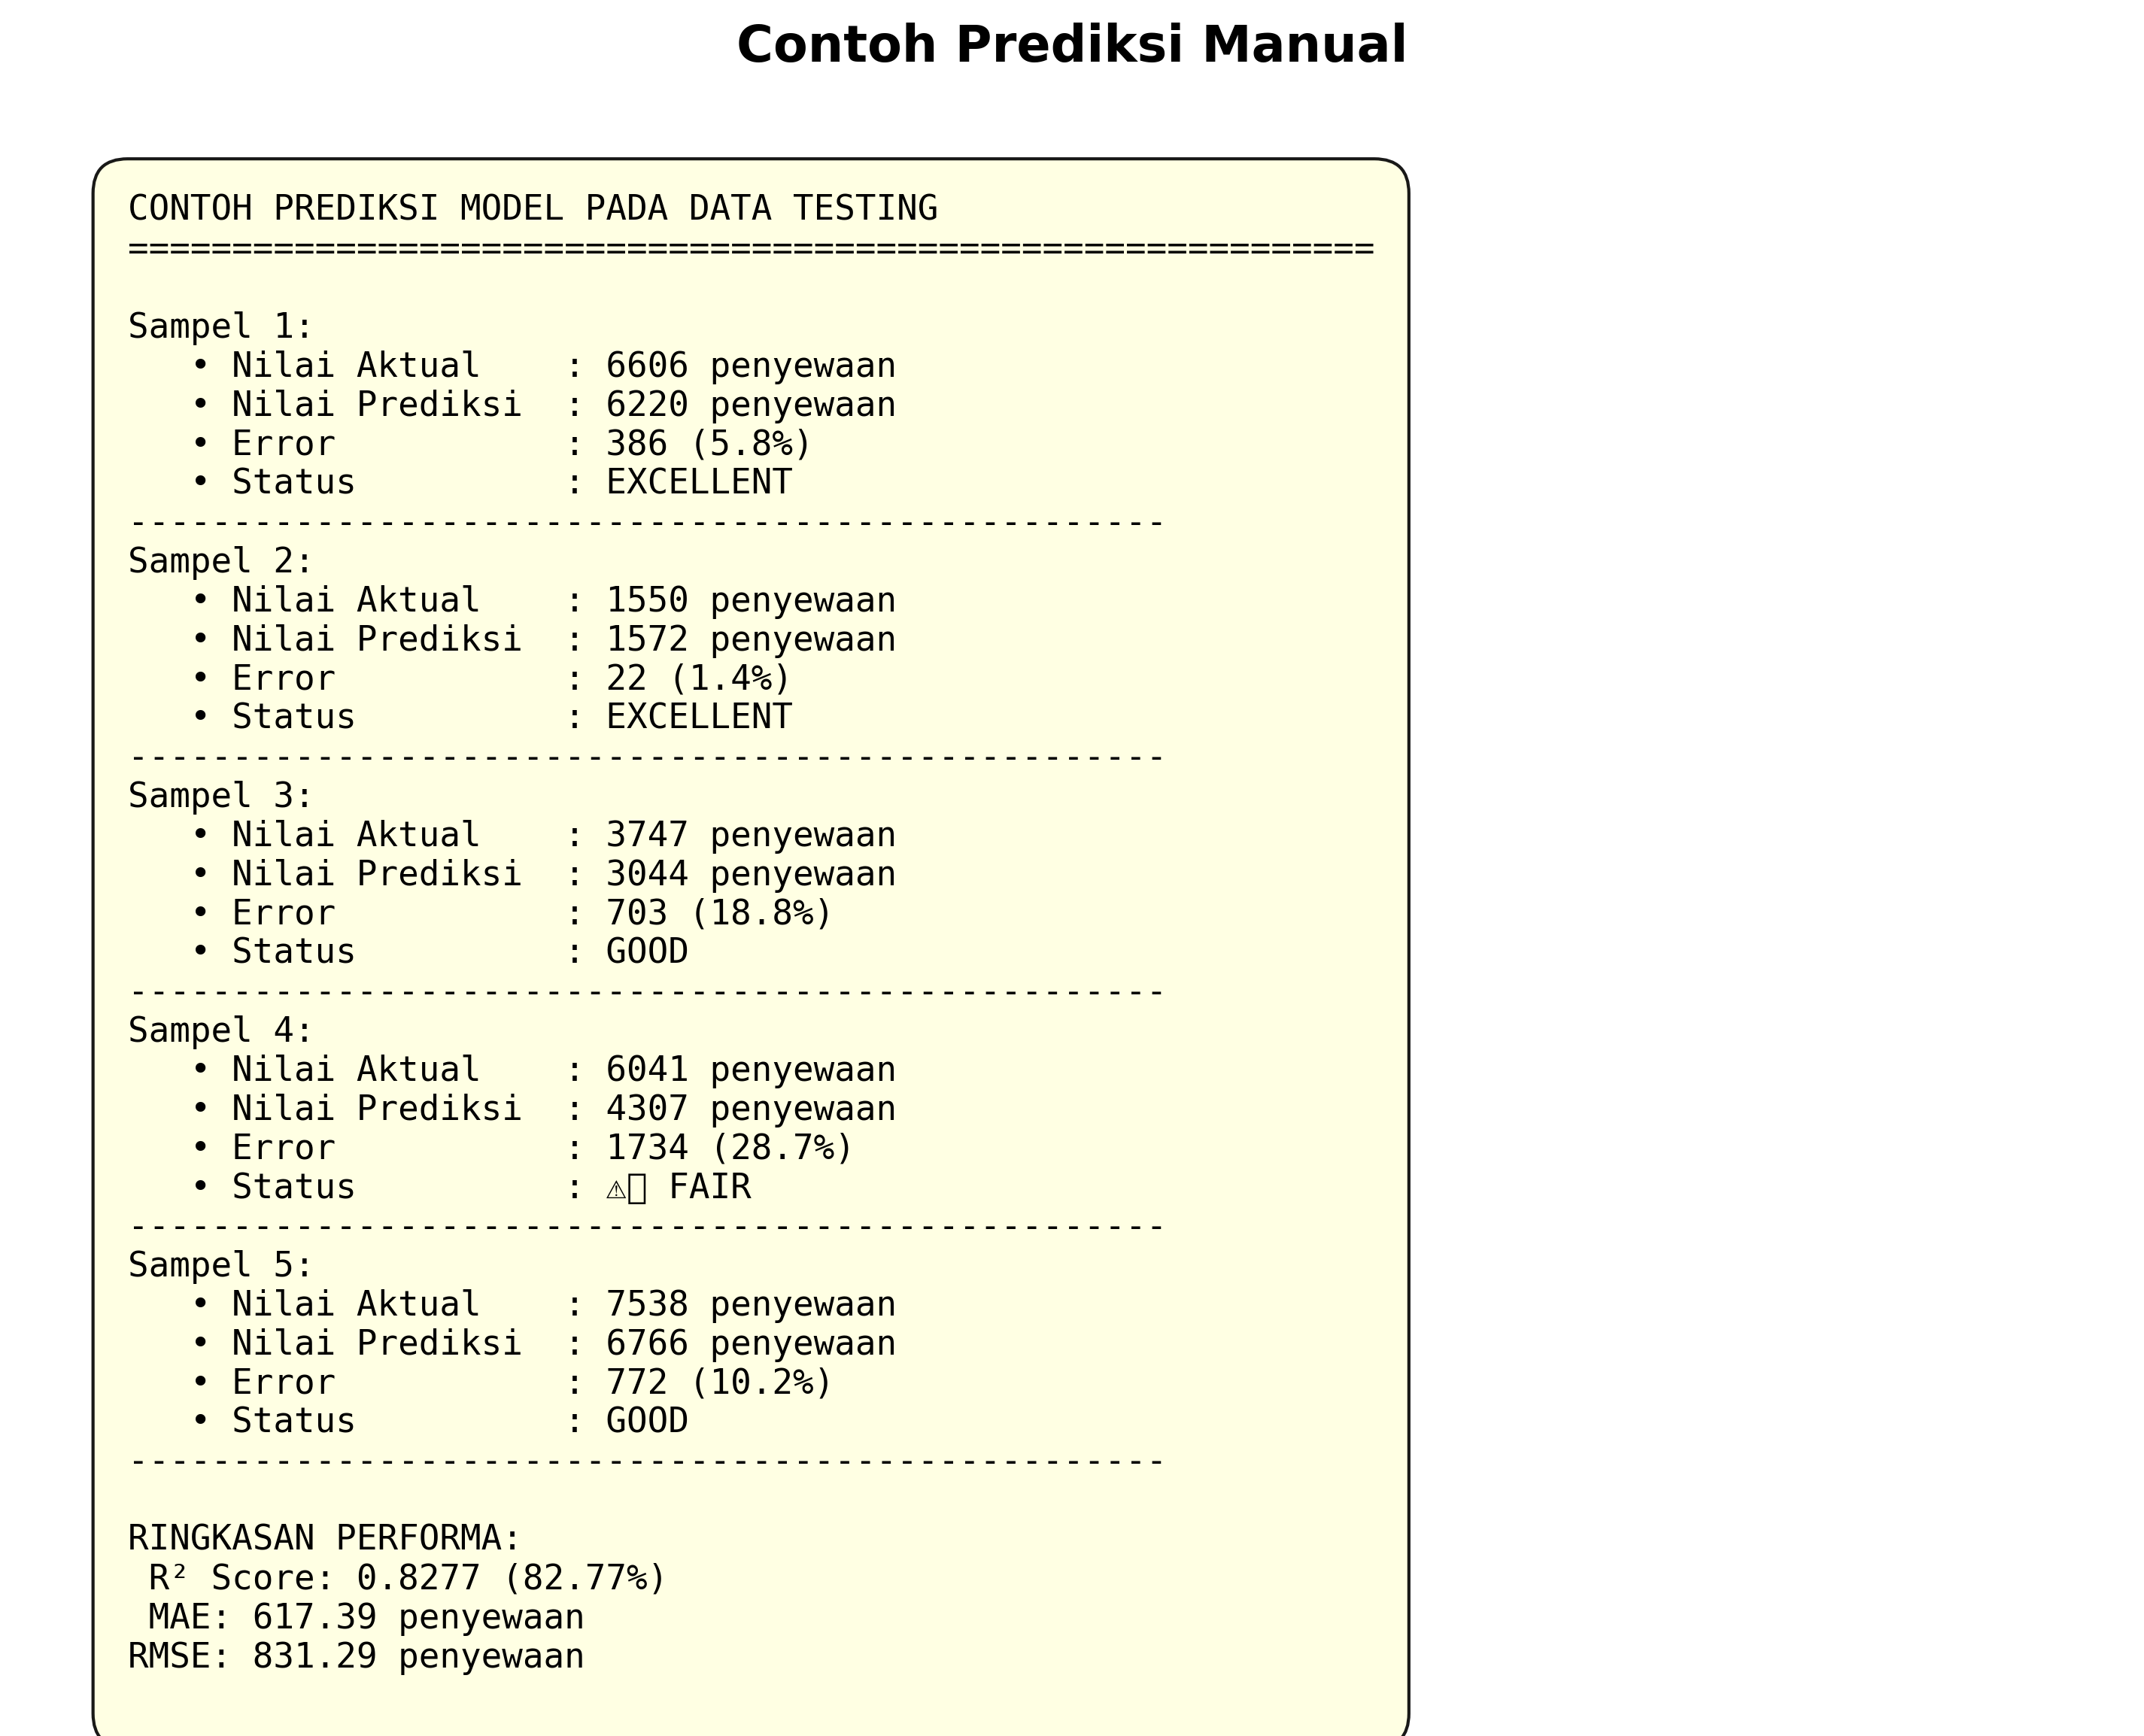
\includegraphics[width=0.8\textwidth]{./OUTPUT/step10_prediction_examples.png}
    \caption{Contoh Prediksi Model pada Data Testing}
    \label{fig:prediction_examples}
\end{figure}

\noindent\textbf{Ikhtisar Prediksi.}
Error bervariasi antara 1{.}4\% hingga 28{.}7\%; mayoritas prediksi akurat untuk penggunaan praktis.

\section{Interpretasi Hasil}
Berdasarkan implementasi Multiple Linear Regression:
\begin{enumerate}
    \item \textbf{Variabel Berpengaruh Positif}: \texttt{atemp} (3488.04), \texttt{temp} (2097.25), \texttt{yr} (2023.99) meningkatkan penyewaan.
    \item \textbf{Variabel Berpengaruh Negatif}: \texttt{windspeed} (-2080.54), \texttt{hum} (-865.44), \texttt{weathersit} (-632.86) menurunkan penyewaan.
    \item \textbf{Kinerja Model}: $R^2$ 82{.}77\% menunjukkan kemampuan prediksi yang sangat baik.
\end{enumerate}

\section{Kesimpulan}
Implementasi Multiple Linear Regression pada dataset Bike Sharing menghasilkan akurasi 82{.}77\%.
Fitur paling berpengaruh adalah suhu (\texttt{temp}, \texttt{atemp}) dan tahun (\texttt{yr}); kelembaban dan kecepatan angin cenderung menurunkan permintaan.
Model dapat dimanfaatkan untuk \textit{forecasting} dan optimasi operasional.

\section{Referensi}
\noindent\textbf{GitHub Repository:}\\
\href{https://github.com/sttnf/machine-learning/tree/main/PERTEMUAN%203/TUGAS/NOTEBOOKS/main.ipynb}{\texttt{PERTEMUAN 3/TUGAS/NOTEBOOKS/main.ipynb}}

\vspace{4pt}
\noindent\textbf{Dataset Source:}\\
\href{https://www.kaggle.com/datasets/lakshmi25npathi/bike-sharing-dataset}{\texttt{Kaggle - Bike Sharing Dataset}}

\end{document}
